\documentclass[11pt,nofonttune,a4paper]{IEEEtran}

\usepackage{amsmath}
%\usepackage{amssymb}
%\usepackage[francais,english]{babel}
%\usepackage{palatino}
\usepackage{gpeyre}
\usepackage{epstopdf}
\usepackage{epsfig}
\usepackage[ruled,vlined]{algorithm2e}

%\usepackage{graphicx}
%\usepackage{epstopdf}
\graphicspath{{./images/}}

% specifics to this paper
\newcommand{\uk}{u^{(k)}}
\newcommand{\tuk}{\tilde u^{(k)}}
\DeclareMathOperator{\Prox}{prox}
\DeclareMathOperator{\Proj}{Proj}
\newcommand{\myparagraph}[1]{\vspace{2mm}\noindent\textbf{#1}}
\newcommand{\tol}{\eta}
\newcommand{\Hm}{\mathcal{H}}
\newcommand{\Um}{\mathcal{U}}
\newcommand{\opnorm}[1]{\big|\!\big|\!\big|#1\big|\!\big|\!\big|}
\DeclareMathOperator{\dom}{dom}

% for the display of algorithms
\usepackage{float}
\floatstyle{boxed}
\floatstyle{ruled}
\newfloat{listing}{H}{loi}
\floatname{listing}{Table}


% FORMAT double interligne
%\renewcommand{\baselinestretch}{1.5}


\begin{document}

% \title{An Algorithm for Total Variation Projection}
\title{Total Variation Projection with First Order Schemes}

\author{
Jalal M. Fadili\thanks{Jalal M. Fadili is with GREYC CNRS-ENSICAEN-Universit\'e de Caen, 
14050 Caen Cedex, France., email: \texttt{jalal.fadili@greyc.ensicaen.fr}} %
and Gabriel Peyr\'e \thanks{Gabriel Peyr\'e is with the CEREMADE CNRS-Universit\'e Paris-Dauphine, 
75775 Paris Cedex 16 France, email: \texttt{gabriel.peyre@ceremade.dauphine.fr}}
}

\markboth{}{Fadili \& Peyr\'e: An Algorithm for Total Variation Projection}

\maketitle

\begin{abstract}
This article proposes a new algorithm to compute the projection on the set of images whose total variation is bounded by a constant. The projection is computed through a dual formulation that is solved by first order non-smooth optimization methods. This yields an iterative algorithm that computes iterative soft thresholding of the dual vector fields, and for which we establish convergence rate on the primal iterates. This projection algorithm can then be used as a building block in a variety of applications such as solving inverse problems under a total variation constraint, or for texture synthesis. Numerical results are reported to illustrate the usefulness and potential applicability of our TV projection algorithm on a variety of examples including denoising, texture synthesis, inpainting and deconvolution problems. We also show that our projection algorithm competes favorably with state-of-the-art TV projection methods in terms of convergence speed.
\end{abstract}

\begin{IEEEkeywords}
Total variation, projection, duality, proximal operator, forward-backward splitting, Nesterov scheme, inverse problems.
\end{IEEEkeywords}

%\IEEEpeerreviewmaketitle
 

%%%%%%%%%%%%%%%%%%%%%%%%%%%%%%%%%%%%%%%%%%%%%%%%%%%%%%%%%%%%%%
%%%%%%%%%%%%%%%%%%%%%%%%%%%%%%%%%%%%%%%%%%%%%%%%%%%%%%%%%%%%%%
%%%%%%%%%%%%%%%%%%%%%%%%%%%%%%%%%%%%%%%%%%%%%%%%%%%%%%%%%%%%%%
\section{Introduction}
\IEEEPARstart{T}{otal} variation is a well known image prior introduced by Rudin, Osher and Fatemi (ROF) \cite{rudin-tv}. For a 
differentiable function $f : \Omega = [0,1]^2 \rightarrow \RR$, it is computed as $\normTV{f} = \int_{\Omega} \abs{\grad f}$, and can be extended to the space $\text{BV}([0,1]^2)$ that contains functions with discontinuities. 

The total variation is used as a regularization to denoise an image $f_0$ by solving the strictly convex problem
\eql{\label{tv-denoising-cont}
	\umin{f \in \text{BV}([0,1]^2)} \frac{1}{2}\norm{f-f_0}^2 + \la \normTV{f},
}
as originally proposed in \cite{rudin-tv}. The regularization weight $\la$ should be tuned to match the noise level contaminating $f_0$.
Several algorithms have been proposed to solve this problem, see for instance \cite{goldfarb-socp-tv,chan-prima-dual-tv,zhu-primal-dual,vogel-iterative-tv,chambolle-algo-tv,weiss-tv-nesterov,AujolTV09,RodriguezTVIRLS09}. Such primal, dual, or primal-dual schemes for denoising are often a building block for solving more complex inverse problems; see e.g. \cite{wang-tv-split,bect-chambolle-iterative}.

\myparagraph{TV projection for denoising.} 
Much less work has focused on denoising an image $f_0$ by projecting it on a total variation ball of radius $\tau < \normTV{f_0}$, which requires to solve\footnote{This constraint set is obviously a closed convex set.}
\eql{\label{tv-proj-cont}
	\umin{\normTV{f} \leq \tau} \norm{f-f_0}.
}
Although there is a bijection between $\lambda$ in \eqref{tv-denoising-cont} and $\tau$ in \eqref{tv-proj-cont} such that the constrained and Lagrangian problems share the same solution, such a bijection is unknown and hard to identify. Thus, the constrained formulation might be preferable over \eqref{tv-denoising-cont} when little is known about the noise level perturbing $f_0$, but when an estimate $\tau$ of the total variation of the clean image is known. For example, such an estimate can be set more easily by relying on some reference (e.g. the observed image itself), and the TV ball radius $\tau$ is set as a {\textit{fraction}} of the TV norm of this reference. Computing the solution of \eqref{tv-proj-cont} with a fast algorithm is thus important for denoising application as has been advocated in \cite{combettes-pesquer-tv}.

An iterative projected sub-gradient method was introduced in \cite{combettes-block,combettes-pesquer-tv}. We propose in this paper a different algorithm that is based on a dual regularization of the primal projection problem. This bears similarities with Chambolle's algorithm \cite{chambolle-algo-tv} that solves the primal TV regularization \eqref{tv-denoising-cont} using a dual projection. Our dual problem is then solved using two first-order iterative schemes: \textit{one-step} forward-backward splitting which dates back to \cite{Gabay83,Tseng91} and recently revitalized in \cite{combettes-splitting}, and accelerated \textit{multi-step} Nesterov scheme \cite{nesterov-gradient}. Both of these algorithms require only the computation of a soft thresholding applied to the dual vector fields at each iteration. Our main theoretical result establishes the convergence rates of the primal iterates of our projection algorithms.

Total variation projection also have far-reaching applications beyond denoising. For example, the extraction of Cheeger sets in landslides modeling \cite{buttazzo-cheeger} can be relaxed as a TV projection problem with boundary constraints, that has been recently solved using sub-gradient projection \cite{carlier-cheeger-numeric}. 

\myparagraph{TV projection for synthesis.} Classical synthesis methods constrain wavelet coefficients \cite{perlin-noise,heeger-pyramid-texture} and are suitable to model some natural phenomena. Computer graphics methods do not rely on statistical modeling and generate a texture through a consistent copy of pixels from an example image \cite{efros-nonparam-sampling,wei-texture-synthesis}. Higher order statistical models \cite{zhu-frame,portilla-parametric-model} improve the visual quality of synthesis by capturing geometric singularities. Section \ref{subsec-texture-synth} shows that a total variation constraint can also be used to enhance the sharpness of edges in texture synthesis. 

\myparagraph{TV projection for inverse problems.}  Total variation projection might be useful as a proxy to solve more challenging inverse problems. Popular linear inverse problems such as inpainting and deconvolution have been the subject of a flurry of research activity where TV has been extensively used to regularize them.

% inpainting
Classical methods for inpainting use partial differential equations that propagate the information from the boundary of the missing region to its interior, see for instance \cite{masnou-level-lines,ballester-filling,bertalmio-inpainting}. Tensor diffusion makes use of a geometric layer to drive the diffusion, see \cite{tschumperle-inpainting}. TV regularization was proposed in \cite{ChanShen01} for inpainting. Sparsity over a redundant frame has also been successfully used to regularize the inpainting problem \cite{starck-inpainting,fadili-inpainting-cj}. 

% deconvolution
There is an extensive literature on the deconvolution problem image processing, and many algorithms have been developed to tackle it. For instance, TV penalty has been used as a regularization term within a variational framework, see e.g. \cite{vogel-iterative-tv-inv,wang-tv-split,bect-chambolle-iterative,ChanTVinverse05,RodriguezTVIRLS09}. Wavelet-based or more generally sparsity-based deconvolution methods have also received considerable attention over the last decade, see e.g. \cite{figueiredo-nowak-em,daubechies-iterated,Combettes2007b,Fadili2006a}.


Inverse problems such as inpainting or deconvolution can be regularized with a total variation constraint \cite{combettes-pesquer-tv}. Sections \ref{subsec-inpainting} and \ref{subsec-deconvolution} are devoted to show how these TV-constrained inverse problems can be solved efficiently using a projected gradient descent iteration, whose projector is computed with our algorithm. 

We would like however stress that this work does not aim to give state-of-the-art results in inverse problems, and instead concentrates on demonstrating how regularization by a TV-ball constraint and the proposed projection algorithms can be harnessed directly to a variety of applications. For instance, denoising will give the same result as TV regularization through the classical ROF model if one is able to identify the appropriate regularization parameter corresponding to the chosen $\tau$ (we recall that there is a bijection between the two parameters). As far as texture synthesis is concerned, our examples are again a proof-of-concept that uses our projection algorithms beside other statistical constraints to produce piecewise-regular textures, hence improving upon existing texture synthesis algorithms such as those proposed in \cite{portilla-parametric-model}.

% Section \ref{subsec-cheeger} shows that this amounts to a constraint projection that can be solved with our method.


\section{Notation and elements of convex analysis}
\label{sec:notation}
Throughout the paper, an image $f$ of $N = n \times n$ pixels is a vector in $\RR^N$. We
denote by $\norm{.}$ the norm induced by the inner product $\dotp{.}{.}$ in $\RR^N$.
We let $\Um = \RR^{N} \times \RR^{N}$ be the space of vector fields with associated inner product $\dotp{u}{v}_\Um = \sum_{0 \leq i,j \leq n-1} (u_1[i,j]v_1[i,j]+u_2[i,j]v_2[i,j])$, $\forall u=(u_1,u_2)$ and $v=(v_1,v_2) \in \Um$. The $\lun$ and $\linf$ norms of a vector field $u=(u_1,u_2) \in \Um$ are respectively $\normu{u} = \sum_{0 \leq i,j \leq n-1} \abs{u[i,j]}$ and $\normi{u} = \umax{i,j} \abs{u[i,j]}$, where $\abs{u[i,j]}:=\sqrt{ u_1[i,j]^2 + u_2[i,j]^2 }$.

Let $C$ a nonempty convex set. The indicator function $\imath_{C}$ of $C$ is 
\eq{
\label{eq:ind}
\imath_{C} (z) =
  \begin{cases}
    0, & \text{if } z \in C ~ ,\\
    +\infty, & \text{otherwise}.
  \end{cases}
}

The domain of a function $\varphi$ is defined by $\dom(\varphi) = \{ z\ :\ \varphi(z) < +\infty \}$ and $\varphi$ is proper if $\dom(\varphi) \neq
\emptyset$. The conjugate of a proper, lower-semicontinuous and convex function $\varphi$ is the proper closed convex function $\varphi^*$ defined by
\eql{
\label{eq:conj}
\varphi^*(z) = \sup_{z \in \dom(\varphi)} \dotp{w}{z} - \varphi(z) ~ ,
}
and we have the bi-conjugate $\varphi^{**}=\varphi$.

The subdifferential of a proper, lower-semicontinuous and convex function $\varphi$ at $z$
is the set-valued map $\partial \varphi$
\eqnl{
\label{eq:subdiff1}
\partial \varphi(z) = \left\{w | \forall v, \varphi(v) \geq \varphi(z) + \dotp{w}{v-z}\right\} ~.
}
An element $w$ of $\partial f$ is called a subgradient. If $\varphi$ is G\^ateaux-differentiable at $z$, its only subgradient is its gradient. A function $\varphi$ is strongly convex with modulus $c > 0$ if and only if
\eqnl{
\label{eq:strongconv}
\varphi(v) \geq \varphi(z) + \dotp{w}{v-z} + \frac{c}{2}\norm{v-z}^2 ~, \forall v ~.
}
See e.g. \cite{LemarechalHiriart96} for comprehensive account on convex analysis and subdifferential calculus.

We also define the notion of a proximity operator, which was introduced in \cite{Moreau1962} as a generalization of convex projection operator. For every $z$, the function $w \mapsto \frac{1}{2}\norm{w-z}^{2} + \varphi(w)$ achieves its infimum at a unique point denoted by $\Prox_{\varphi}z$. The uniquely-valued operator $\Prox_{\varphi}$ thus defined is the \textit{proximity operator} of $\varphi$.


%%%%%%%%%%%%%%%%%%%%%%%%%%%%%%%%%%%%%%%%%%%%%%%%%%%%%%%%%%%%%%
%%%%%%%%%%%%%%%%%%%%%%%%%%%%%%%%%%%%%%%%%%%%%%%%%%%%%%%%%%%%%%
%%%%%%%%%%%%%%%%%%%%%%%%%%%%%%%%%%%%%%%%%%%%%%%%%%%%%%%%%%%%%%
\section{Discrete Dual Formulation}

The optimization \eqref{tv-proj-cont} is computed numerically by discretizing the gradient operator and the total variation to project an image of $N = n \times n$ pixels.

%%%%%%%%%%%%%%%%%%%%%%%%%%%%%%%%%%%%%%%%%%%%%%%%%%%%%%%%%%%%%%
\subsection{Discrete Total Variation}

A discretized gradient for an image $f \in \RR^N$ is defined as $\grad f[i,j] = (\partial_x f[i,j],\partial_y f[i,j])$, where
\begin{align*}
	\partial_x f[i,j]& = 
	\choice{
		f[i+1,j]-f[i,j] \qifq 0 \leq i < n-1,\\
		0 \text{ otherwise,}
	}\\
	\partial_y f[i,j]& = 
	\choice{
		f[i,j+1]-f[i,j] \qifq 0 \leq j < n-1,\\
		0 \text{ otherwise}.
	}
\end{align*}
The gradient is thus a vector field $\grad f \in \Um$. The discrete total variation is $\normTV{f} = \normu{\grad f}$ where the $\lun$ norm of a vector field in $\Um$ is defined in Section~\ref{sec:notation}.

The adjoint of the gradient is $\grad^* = -\diverg$, where the divergence of a vector field $u = (u_1,u_2) \in \Um$ is
$\diverg(u) = \partial_x^* u_1 + \partial_x^* u_2$, with
\begin{align*}
	\partial_x^* f[i,j]& = 
	\choice{
		f[i,j]-f[i-1,j] \qifq 0 < i < n,\\
		0 \text{ otherwise,}
	}\\
	\partial_y^* f[i,j]& = 
	\choice{
		f[i,j]-f[i,j-1] \qifq 0 < j < n,\\
		0 \text{ otherwise}.
	}
\end{align*}

%%%%%%%%%%%%%%%%%%%%%%%%%%%%%%%%%%%%%%%%%%%%%%%%%%%%%%%%%%%%%%
\subsection{Total Variation Projection}

The goal of this paper is to compute the projection $f^\star$ of an image $f_0$ on a set of images with bounded variation
\eql{\label{eq-primal}
	f^\star = \uargmin{f \in \RR^N, \, \normTV{f} \leq \tau} \norm{f-f_0}^2.
}	
where $0 < \tau < \normTV{f_0}$ to avoid the trivial solution $f^\star = f_0$.

The following proposition shows that the primal constrained optimization problem \eqref{eq-primal} is recast into a penalized form.

\begin{prop}
\label{prop:dualmin}
	For any $f \in \RR^N$, the primal solution is recovered as $f^\star = f_0 - \diverg(u^\star)$ where $u^\star$ is the solution of the dual problem
	\eql{\label{eq-dual}
		\inf_{u \in \RR^{N \times 2}} \frac{1}{2} \norm{f_0 - \diverg(u)}^2 + \tau \normi{u} ~.
	}
\end{prop}
\begin{IEEEproof}
Let's introduce the dual variable $u \in \Um$. First, it is easy to show that the Fenchel conjugate of the $\linf$ norm is the indicator function of the $\lun$ norm. Indeed, by the H\"older inequality we have $\dotp{u}{v}_\Um \leq \norm{u}_\infty\norm{v}_1$~\footnote{An alternative proof can be found in e.g. \cite[Proposition V.3.2.1]{LemarechalHiriart96}.}, we then get
\begin{eqnarray*}
\pa{\tau\normi{.}}^*(v)&=& \sup_{u \in \Um}~ \dotp{u}{v}_\Um - \tau\normi{u} \\
			     &=& \sup_{\rho > 0}\sup_{\normi{u}=\rho} \dotp{u}{v}_\Um - \tau\rho \\
			     &=& \sup_{\rho > 0}\rho\pa{\norm{v}_1 - \tau} = \imath_{\{\norm{\cdot}_1 \leq \tau\}}(v) ~.
\end{eqnarray*}

Thus, using the bi-conjugate relation, one can write the TV-ball indicator function as
\eq{
\imath_{\{\normTV{\cdot} \leq \tau\}}(f) = \sup_{u \in \Um}~ \dotp{u}{\grad f}_\Um - \tau \normi{u}.
}
This allows to rewrite \eqref{eq-primal} as
\eqnl{\label{eq-proof-dual-1}
\umin{f\in \RR^N} \frac{1}{2}\norm{f-f_0}^2 + \imath_{\{\normTV{\cdot} \leq \tau\}}(f) 
&=& \sup_{u \in \Um}~  - \tau \normi{u} + \umin{f \in \RR^N} \dotp{u}{\grad f}_\Um + \frac{1}{2}\norm{f-f_0}^2 ~\nonumber \\
&=& - \inf_{u \in \Um}~ \tau \normi{u} - \umin{f \in \RR^N} -\dotp{\diverg(u)}{f}  + \frac{1}{2}\norm{f-f_0}^2 ~.
}
The inner minimization involves a strongly convex function, whose unique primal solution $f^\star$ is recovered from the dual variable $u$ as
\eql{
\label{eq:primaldualgrad}
f^\star = \uargmin{f \in \RR^N} -\dotp{\diverg(u)}{f} + \frac{1}{2}\norm{f-f_0}^2 = f_0 + \diverg(u),
}
and
\eql{\label{eq-proof-dual-2}
-\dotp{\diverg(u)}{f^\star} + \frac{1}{2}\norm{f^\star-f_0}^2 = - \frac{1}{2}\norm{ f_0 + \diverg(u) }^2+\frac{1}{2}\norm{f_0}^2 ~.
}

Combining \eqref{eq-proof-dual-1} and \eqref{eq-proof-dual-2} with the obvious change of sign on $u$ leads to the optimization problem \eqref{eq-dual}.
	
\end{IEEEproof}

\begin{rem}
Proposition~\ref{prop:dualmin} can be alternatively proved using Fenchel-Rockafellar duality formula well-known in convex analysis, see e.g. \cite[Section III.4]{Ekeland74}. We have chosen this line of proof for convenience and the sake of accessibility to the reader.
\end{rem}

%%%%%%%%%%%%%%%%%%%%%%%%%%%%%%%%%%%%%%%%%%%%%%%%%%%%%%%%%%%%%%
%%%%%%%%%%%%%%%%%%%%%%%%%%%%%%%%%%%%%%%%%%%%%%%%%%%%%%%%%%%%%%
%%%%%%%%%%%%%%%%%%%%%%%%%%%%%%%%%%%%%%%%%%%%%%%%%%%%%%%%%%%%%%
\section{First-Order Schemes on the Dual Problem}
\label{sec-1storder}

In going from the primal problem \eqref{eq-primal} to the dual formulation \eqref{eq-dual}, we have replaced a constrained problem with an unconstrained penalized form. The primal solution is easily recovered from the dual solution as $f^\star = f_0 - \diverg(u^\star)$. Furthermore, it turns out that the dual problem \eqref{eq-dual} is easier to solve with various first order non-smooth optimization schemes. Indeed, \eqref{eq-dual} involves a quadratic form which has a Lipschitz continuous gradient, and the non-differentiable $\linf$ term. Section \ref{subsec-fb} presents a \textit{one-step} forward-backward splitting iteration, as explained for instance in \cite{Tseng91,combettes-splitting}, while Section \ref{subsec-nesterov} proposes an accelerated \textit{multi-step} scheme due to Nesterov, see \cite{nesterov-gradient} and also \cite{weiss-tv-nesterov} for some applications to image processing. It turns out that both these algorithms involve the computation of the proximity operator associated to the $\linf$ norm that can be computed explicitly as explained in the following section.

%Such methods are designed to optimize the sum of a smooth functional, here $\frac{1}{2}\norm{f_0 - \diverg(u)}^2$ and a non-smooth functional, here $\normi{u}$. They compute iterated vector fields $\uk$ that converge to the solution $u^{(+\infty)} = u^\star$ of \eqref{eq-dual}. 

%%%%%%%%%%%%%%%%%%%%%%%%%%%%%%%%%%%%%%%%%%%%%%%%%%%%%
\subsection{$\linf$ Proximity Operator}
\label{subsec-proximal}

Recall from Section~\ref{sec:notation} that the proximity operator $\Prox_{\kappa \normi{\cdot}}(u)$ associated to $\kappa \normi{\cdot}$ amounts to solving
\eql{\label{eq-proximal-inf}
	\Prox_{\kappa \normi{\cdot}}(u) = \uargmin{ v \in \Um } \frac{1}{2} \norm{u-v}^2 + \kappa \normi{v}.
}
Proposition \ref{prop-soft-thresh} hereafter shows that $\Prox_{\kappa \normi{\cdot}}(u)$ is computed explicitly through a soft thresholding $S_\la$ applied on the dual vector field $u$ for a properly chosen value of $\la$. 

To get the precise value of $\la$ for a given vector field $u \in \Um$, we need to compute $d[0] \leq d[1] \leq \ldots \leq d[N-1]$ that orders the set of norms
\eql{\label{eq-def-d}
	\{d[t]\}_{t=0}^{N-1} = \{ \abs{u[i,j]} \}_{i,j=0}^{n-1}, 
}
and also the cumulated ordered norms
\eql{\label{eq-def-D}
	D[s] = \sum_{t=s+1}^{N-1} d[t].
}

\begin{prop}\label{prop-soft-thresh}
	For $u \in \Um$, with $d$ and $D$ as defined in \eqref{eq-def-d}-\eqref{eq-def-D}, we have $\Prox_{\kappa \normi{\cdot}}( u ) = 0$ if $\normu{u} \leq \kappa$ and $\Prox_{\kappa \normi{\cdot}}( u ) = u - S_\la(u)$ otherwise, where
	\eql{\label{eq-soft-thresh}
		S_\la(u)[i,j] = \max\pa{ 1 - \frac{\la}{\abs{ u[i,j] }} , 0 } u[i,j]
	}
	and $\la > 0$ is given by 
	\eql{\label{eq-defn-la}
		\la = d[t] + (d[t+1]-d[t]) \frac{D[t+1] - \kappa}{ D[t+1] - D[t] }
	}
	where $t$ is such that $D[t+1] \leq \kappa < D[t]$.	
\end{prop}
\begin{IEEEproof}
Using a similar proof to that of Proposition~\ref{prop:dualmin}, we have the relation between the primal and dual minimization problems
\eqn{
\Prox_{\kappa \normi{\cdot}}( u ) = \uargmin{v \in \Um} \frac{1}{2} \norm{u-v}^2 + \kappa \normi{v} \iff  \Proj_{\{\normu{\cdot} \leq \kappa\}}(u) = \uargmin{w \in \Um} \frac{1}{2}\norm{u-w}^2 + \imath_{\{\normu{\cdot} \leq \kappa\}}(w) ~.
}
where $\Proj_{\{\normu{\cdot} \leq \kappa\}}(u)$ is the orthogonal projection of $u$ onto the closed $\lun$ ball in $\Um$ of radius $\kappa$. In the same vein as \eqref{eq:primaldualgrad}, the relation between the primal and dual solutions (both are unique here) yields
\eql{
\label{eq:proxproj}
\Prox_{\kappa \normi{\cdot}}( u ) = u - \Proj_{\{\normu{\cdot} \leq \kappa\}}(u) ~.
}
If $\normu{u} \leq \kappa$, then $\Prox_{\kappa \normi{\cdot}}( u ) = 0$. Otherwise, the projection $\Proj_{\{\normu{\cdot} \leq \kappa\}}(u)$ is computed by finding the Lagrange multiplier $\lambda(\kappa)$ such that
\eql{
\label{eq:softlagrangian}
	\Proj_{\{\normu{\cdot} \leq \kappa\}}(u) = \uargmin{ v } \frac{1}{2} \norm{u-v}^2 + \la(\kappa) \normu{v}.
}
As noticed for instance in \cite{chambolle-wavelets} for wavelet thresholding, the solution of \eqref{eq:softlagrangian} has a closed-form known as soft-thresholding extended to vector fields
\eq{
	\Proj_{\{\normu{\cdot} \leq \kappa\}}(u) = S_{\la(\kappa)}(u).
}

Observe that $\normu{S_{\la}(u)} = \sum_{\abs{u[i,j]} > \la} \pa{\abs{u[i,j]} - \la}$ is a piecewise affine and decreasing function of $\lambda$ with slope changing at the ordered values $d[t]$. One can then check that the value of $\la$ that meets the constraint $\normu{S_{\la}(u)}=\kappa$ is the one given by \eqref{eq-defn-la}.
\end{IEEEproof}

Our result bears similarities with that of \cite{chambolle-wavelets} who use different arguments to compute the proximity operator of the Besov norm $\mathbf{B}^1_{\infty,1}$. In words, Proposition~\ref{prop-soft-thresh} tells us that the proximity operator of the $\linf$-norm of a vector field $u \in \Um$ is computed by sorting its magnitudes, which of course can be done in $O(N\log N)$ expected time. A similar ingredient appear in the projection on the $\lun$-ball for scalar fields as in \cite{candes-practical,daubechies-projected}. An improved approach replaces sorting with a median-search-like procedure whose expected complexity is linear in $N$, this has been rediscovered independently in \cite{Duchi08} and \cite{berg-group}.

\begin{rem}
Equation \eqref{eq:proxproj} can be proved alternatively using Moreau decomposition which allows to conclude that $\Prox_{\varphi^*}( u ) = u - \Prox_{\varphi}(u)$, see for instance \cite{Moreau1965} and \cite[Lemma 2.10]{combettes-splitting}.
\end{rem}

%%%%%%%%%%%%%%%%%%%%%%%%%%%%%%%%%%%%%%%%%%%%%%%%%%%%%
\subsection{Forward-backward Projection Algorithm}
\label{subsec-fb}

The projection $f^\star = f_0 - \diverg(u^\star)$ is computed by solving the dual unconstrained optimization problem \eqref{eq-dual}. Owing to Lipschitz differentiability of the quadratic term, the dual problem verifies the necessary prerequisite to be solved with the one-step forward-backward splitting recursion. 

The forward-backward scheme can be written in a compact form with descent step-size $\mu > 0$ \footnote{The descent step-size can be even a sequence $\mu_k>0$ that varies from one iteration to another.} 
\eql{\label{eq-proximal-iteration}
	u^{(k+1)} = \Prox_{\mu \tau\normi{\cdot}}\left(\uk - \mu \grad\pa{ f_0 - \diverg(\uk) }\right),
}
where the proximity operator for $\kappa=\mu\tau$ is defined in \eqref{eq-proximal-inf}. The overall algorithm to minimize \eqref{eq-primal} is summarized in Algorithm~\ref{algorithm-tv-proj}.

{\linespread{1}
\begin{algorithm}[h]
\noindent{\bf{Initialization:}} choose some $u^{(0)} \in \Um$, $\mu \in (0,1/4)$, set $k=0$. \\
\noindent{\bf{Main iteration:}} \\
\While{$\norm{u^{(k+1)} - u^{(k)}} > \tol$}{
\begin{enumerate}
	\item \textit{Gradient descent step:} compute
	\eq{
		\tuk = \uk - \mu \grad\pa{ f_0 - \diverg(\uk) }.
	}
	\item \textit{TV correction step:} compute $d$ and $D$ as defined in \eqref{eq-def-d} and \eqref{eq-def-D} and set $\la$ as in \eqref{eq-defn-la} with $\kappa=\mu\tau$. Define
		\eq{
			u^{(k+1)} = \tuk - S_\la( \tuk ),	
		}
		using the soft thresholding operator \eqref{eq-soft-thresh}.
	\item $k=k+1$.
\end{enumerate}}
\noindent{\bf{Output:}} $f^\star = f_0 - \diverg(u^{(k+1)})$.
\caption{Forward-backward total variation projection. \label{algorithm-tv-proj}}
\end{algorithm}}

\subsubsection{Convergence analysis}
Theorem~\ref{theo:convFB} ensures that the sequence $(f^{(k)})_{k \in \NN}$ obtained from Algorithm~\ref{algorithm-tv-proj} converges to the solution of \eqref{eq-primal} with a convergence rate $O(1/k)$.
\begin{thm}
\label{theo:convFB}
Suppose that $\mu \in (0,1/4)$. Let $u^{(0)} \in \RR^{N \times 2}$. The sequence of iterates $f^{(k)} = f_0 - \diverg(\uk)$, where $\uk$ is the dual sequence in \eqref{eq-proximal-iteration}, converges to $f^\star$. More precisely, there exists a $C > 0$ such that
\[
\norm{f^{(k)}-f^\star}^2 \leq C/k.
\]
\end{thm}

\begin{IEEEproof}
By coercivity, the set of solutions of \eqref{eq-dual} is non empty. Moreover, let $\opnorm{\diverg}$ be the operator norm of the discrete divergence. The term $\norm{f_0 - \diverg(u)}^2/2$ is differentiable whose gradient is Lipschitz continuous with Lipschitz constant $\opnorm{\diverg}^2 \leq 8$ \cite{chambolle-algo-tv}. Thus, by continuity of the mapping $u \mapsto f=f_0 - \diverg(u)$, and since the projection $f^\star$ is unique, applying \cite[Corollary~6.5]{combettes-monotone-inclusions}, we deduce that the sequence of iterates $f^{(k)}$ converges to $f^\star$ provided that the step-size satisfies $0 < \underline{\mu} \leq \mu \leq \overline{\mu} < 1/4 \leq 2/\opnorm{\diverg}^2$.

Let's now turn to the convergence rate. We let $J(f)$ and $\tilde{J}(u)$ be the primal and the dual objectives given in \eqref{eq-primal} and \eqref{eq-dual}, namely
\eql{
\label{eq:primaldualobj}
\begin{split}
J(f)         &= \underset{H(f)}{\underbrace{\frac{1}{2} \norm{f - f_0}^2}} + \underset{G(\grad f)}{\underbrace{\imath_{\{\normTV{.} \leq \tau\}}(f)}}, \\
\tilde{J}(u) &= \underset{H^*(\diverg(u))}{\underbrace{\frac{1}{2} \norm{f_0 - \diverg(u)}^2 - \frac{1}{2}\norm{f_0}^2}} + \underset{G^*(u)}{\underbrace{\tau\normi{u}}} ~,
\end{split}
}
where $H^*$ and $G^*$ are the conjugates of $H$ and $G$ respectively. Recall that from Proposition~\ref{prop:dualmin}, we have
\eqnl{
\label{eq:primaldualineq}
\min_{f}~ J(f) = - \inf_u~ \tilde{J}(u) \iff J(f) \geq J(f^\star) = -\tilde{J}(u^\star) \geq -\tilde{J}(u) \quad \forall ~ (f,u) \in \RR^N \times \Um ~,
}
and from the primal-dual solutions relationship
\eqnl{
\label{eq:primaldualfenchel}
H(f^\star) + H^*(\diverg(u^\star)) = \dotp{f^\star}{\diverg(u^\star)} \iff f^\star = (\Diffu H^*) (\diverg(u^\star)) ~,
}
where $\Diffu H^*$ is the gradient of $H^*$ with respect to $u$.

We introduce the following two notions which are essential to prove the convergence rate of our scheme. First, for an optimal solution $u^\star \in \Um$, we define the Bregman-like distance as the functional
\eqnl{
B(v) = G^*(v) - G^*(u^\star) + \dotp{-\grad(\Diffu H^*)(\diverg(u^\star))}{v-u^\star}_\Um ~, ~ \forall ~ v \in \Um ~.
}
This is indeed a distance-like function to $u^\star$ since $B(v)$ is non-negative and $B(u^\star)=0$. $B(v)$ is non-negative by applying the subgradient inequality \eqref{eq:subdiff1} to $G^*$ since the minimality condition corresponding to \eqref{eq-dual} is equivalent to the inclusion $\grad(\Diffu H^*)(\diverg(u^\star)) \in \partial G^*(u^\star)$. The Bregman distance is widely used to analyze properties of descent algorithms, see \cite{Bauschke03,BrediesLorentz08} and references therein.

Additionally, as $H^*$ is differentiable, we define the Taylor distance as the remainder of the 1st order Taylor expansion of $H^*$ at $u^\star$
\eqnl{
T(v) = H^*(\diverg(v)) - H^*(\diverg(u^\star)) - \dotp{-\grad(\Diffu H^*)(\diverg(u^\star))}{v-u^\star}_\Um ~, ~ \forall ~ v \in \Um ~.
}
This is again a non-negative function ($H^*$ is convex), and $T(u^\star)=0$. 

It is not difficult to see that these functionals verify the following property
\eqnl{
B(\uk)+T(\uk) = \tilde{J}(\uk) - \tilde{J}(u^\star) ~.
}
Since the function $H^*(f)=\norm{f-f_0}^2/2$ is strongly convexity of modulus 1, and using \eqref{eq:primaldualfenchel}, we have
\eqnl{
\label{eq:strongconvexT}
T(\uk) &=& H^*(\diverg(\uk)) - H^*(\diverg(u^\star)) - \dotp{-\grad(\Diffu H^*)(\diverg(u^\star))}{\uk-u^\star}_\Um \nonumber \\
       &=& H^*(\diverg(\uk)) - H^*(\diverg(u^\star)) - \dotp{(\Diffu H^*)(\diverg(u^\star))}{\diverg(\uk)-\diverg(u^\star)} \nonumber \\
       &=& \frac{1}{2}\norm{\diverg(\uk)-\diverg(u^\star)}^2 = \frac{1}{2}\norm{f^{(k)}-f^\star}^2 ~.
}
Using \cite[Theorem~4]{nesterov-gradient}, the convergence rate over $\tilde{J}$ is such that
\eqnl{
\label{eq:rateFBdualobj}
\tilde{J}(\uk) - \tilde{J}(u^\star) &\leq& \frac{2\opnorm{\diverg}^2R^2}{k+2} ~, \quad \forall ~ k \geq 0 ~,
}
where $R$ is the radius of the sublevel sets of $\tilde{J}$, i.e. $R=\umax{u: \tilde{J}(u) \leq \tilde{J}(u^{(0)})} \norm{u - u^\star} < +\infty$.

Thus, by positivity of $B(\uk)$, and $\opnorm{\diverg}^2 \leq 8$
\eqnl{
\label{eq:rateFBT}
T(\uk) \leq \tilde{J}(\uk) - \tilde{J}(u^\star) \leq \frac{16 R^2}{k+2} ~, \quad \forall ~ k \geq 0 ~.
}
Piecing together \eqref{eq:strongconvexT} and \eqref{eq:rateFBT}, we obtain
\eqnl{
\label{eq:rateFBprimal}
\norm{f^{(k)} - f^\star}^2 &\leq& 2T(\uk) \nonumber\\
&\leq& \frac{32 R^2}{k+2}~, \quad \forall ~ k \geq 0 ~,
}
which gives the desired rate.
\end{IEEEproof}

\begin{rem}
\begin{itemize}
\item It is important to note that the above proof is general and applies to any problem in the form \eqref{eq:primaldualobj} beyond the TV projection problem considered here, provided that $H^*$ is strongly convex with Lipschitz continuous gradient, or by properties of the conjugate that $H$ is strongly convex and has a Lipschitzian gradient \cite[Theorem~4.2.1 and 4.2.2]{LemarechalHiriart96}. Strong convexity is of course important to derive the rate \eqref{eq:rateFBprimal} over the primal iterates, but the rate on the dual objective in \eqref{eq:rateFBdualobj} remains valid anyway. Note that the equality \eqref{eq:strongconvexT} becomes a lower-bound inequality for general strongly convex $H^*$, with a constant involving the strong convexity modulus and the Lipschitz constant. 
\item We point out that another proof of the convergence rate of the forward-backward splitting in terms of the objective has recently appeared in \cite[Proposition~2]{BrediesLorentz08}. The rate of \cite{nesterov-gradient} is nevertheless sharper.
\end{itemize}
\end{rem}

This result asserts that Algorithm~\ref{algorithm-tv-proj} necessitates as large as $O(1/\eta)$ iterations to reach a $\eta$ convergence tolerance on the iterates.

%%%%%%%%%%%%%%%%%%%%%%%%%%%%%%%%%%%%%%%%%%%%%%%%%%%%%
\subsection{Multi-step Projection Algorithm}
\label{subsec-nesterov}
In \cite{nesterov-gradient,nesterov-smooth}, Nesterov proposes an accelerated multi-step gradient algorithm to solve functionals formed as a sum of two convex terms: a smooth one with Lipschitz-continuous gradient and a non-necessarily smooth term whose structure is simple. By simple, we intend in our context that the corresponding proximity operator is accessible. The dual problem \eqref{eq-dual} falls within the scope of the Nesterov algorithm. Unlike the forward-backward iteration \eqref{eq-proximal-iteration}, Nesterov accelerated version uses explicitly all previous iterates $u^{(i)}$, $i < k$ to compute $\uk$, hence the name multi-step algorithm.

Algorithm~\ref{algorithm-tv-proj-nesterov} details the steps of Nesterov scheme to minimize \eqref{eq-dual}. It is formulated using proximal operators, as described in \cite{weiss-tv-nesterov}. 

{\linespread{1}
\begin{algorithm}[h]
\noindent{\bf{Initialization:}} $u^{(0)} \in \Um$, $A_0=0$, $\xi^{(0)}=0$, $\mu \in (0,1/4)$. \\
\noindent{\bf{Main iteration:}} \\
\While{$\norm{u^{(k+1)} - u^{(k)}} > \tol$}{
\begin{enumerate}
\item \textit{First proximal computation:} 
\eq{
\upsilon^{(k)} = \Prox_{A_k \tau \normi{\cdot}}(u^{(0)} - \xi^{(k)}) ~, 
}
where the proximal operator is computed as defined in Proposition \ref{prop-soft-thresh} with $\kappa=A_k\tau$.
\item Set $a_k = \pa{\mu + \sqrt{\mu^2 + 4\mu A_k}}/2$ and $\omega^{(k)} = \frac{ A_k\uk + a_k \upsilon^{(k)} }{ A_k + a_k }$. \\
\item \textit{Second proximal computation:}
\eqn{
\tilde \omega^{(k)} &=& \omega^{(k)} - \frac{\mu}{2} \grad\pa{ f_0 - \diverg(\omega^{(k)}) },\\
u^{(k+1)} &=& \Prox_{\mu \tau / 2 \normi{\cdot}}( \tilde \omega^{(k)} ) ~ ,
}
where the proximal operator is computed as defined in Proposition \ref{prop-soft-thresh} with $\kappa=\mu \tau / 2$.
\item Update $A_{k+1} = A_k+a_k$ and $\xi^{(k+1)} = \xi^{(k)} + a_k \grad\pa{ f_0 - \diverg(u^{(k+1)}) }$.
\item $k=k+1$.
\end{enumerate}
}
\noindent{\bf{Output:}} $f^\star = f_0 - \diverg(u^{(k+1)})$.
\caption{Nesterov total variation projection. \label{algorithm-tv-proj-nesterov}}
\end{algorithm}}


\subsubsection{Convergence analysis}
The following results gives the convergence rate of the primal sequence $f^{(k)} = f_0 - \diverg(\uk)$ obtained from Algorithm~\ref{algorithm-tv-proj-nesterov}.
\begin{thm}
\label{theo:convnesterov}
Suppose that $\mu \in (0,1/4)$. Let $u^{(0)} \in \RR^{N \times 2}$. Then, after $k$ iterations, the sequence of iterates $(f^{(k)})_{k \geq 1}$ is such that $\exists~C > 0$
\[
\norm{f^{(k)}-f^\star}^2 \leq C/k^2.
\]
\end{thm}

\begin{IEEEproof}
The proof of this result is patterned after that of Theorem~\ref{theo:convFB} starting at \eqref{eq:rateFBdualobj}. Indeed, by virtue of \cite[Theorem~6]{nesterov-gradient}, and $\opnorm{\diverg}^2 \leq 8$, we arrive at
\eqnl{
\label{eq:rateNestdualobj}
\tilde{J}(\uk) - \tilde{J}(u^\star) \leq  \frac{32 R^2}{k^2} ~, \quad k \geq 1 ~,
}
where now $R=\norm{u^\star - u^{(0)}}^2$.
Finally, from \eqref{eq:strongconvexT}, we deduce the desired rate
\eqnl{
\label{eq:ratenestprimal}
\norm{f^{(k)} - f^\star}^2 \leq \frac{64 R^2}{k^2} ~, \quad k \geq 1 ~.
}
\end{IEEEproof}

\begin{rem}
Again, in the same vein as the proof of Theorem~\ref{theo:convFB}, the above proof is general and applies straightforwardly to any problem in the form \eqref{eq:primaldualobj} beyond TV projection, with the proviso that $H^*$ is strongly convex to get the rate on the iterates. For the case where $H^*$ is not necessarily strongly convex, but has a bounded domain, the convergence rate over the primal objective was established in \cite[Theorem~3]{nesterov-smooth} and \cite{weiss-phd}. The latter followed the same lines of proof as the former.
\end{rem}

This result asserts that Algorithm~\ref{algorithm-tv-proj-nesterov} necessitates only $O(1/\sqrt{\tol})$ iterations to reach a $\tol$-convergence tolerance both on the primal iterates and objective. This is much faster than $O(1/\tol)$ iterations required by the forward-backward scheme.

%%%%%%%%%%%%%%%%%%%%%%%%%%%%%%%%%%%%%%%%%%%%%%%%%%%%%%%%%%%%%%
%%%%%%%%%%%%%%%%%%%%%%%%%%%%%%%%%%%%%%%%%%%%%%%%%%%%%%%%%%%%%%
%%%%%%%%%%%%%%%%%%%%%%%%%%%%%%%%%%%%%%%%%%%%%%%%%%%%%%%%%%%%%%
\section{Inverse Problems}

Image acquisition devices compute $P \leq N$ noisy indirect measurements 
\eql{\label{eq-ip-inversion}
	y = \Phi f_0 + \epsilon \in \RR^p.
}
of an image $f_0 \in \RR^N$, where $\epsilon$ is an additive noise.
The linear bounded operator $\Phi$ typically accounts for blurring, sub-sampling or missing pixels so that the measured data $y$ only captures a small fraction of the original image $f$ one wishes to recover.

%%%%%%%%%%%%%%%%%%%%%%%%%%%%%%%%%%%%%%%%%%%%%%%%%%%%%%%%%%%%%%
\subsection{Regularization with TV Constraint}

A total variation prior allows to to regularize the solution by reducing the space of candidate solutions of the inverse problem to those belonging to a total variation ball of finite radius. Thus solving such a constrained inverse problem provides an image that both matches approximately the forward measurements $y$ and that has a low total variation. If the noise is assumed to be zero-mean of finite variance, it is devised to solve the constrained optimization problem
\eql{\label{tv-ip-constr}
	\umin{f \in \RR^N} \normTV{f}
	\qsubjq
	\norm{y - \Phi f} \leq \gamma
}
where $\gamma$ is related to the noise standard deviation supposedly known a priori. 

On the contrary, if a little is known about the noise $\epsilon$, but one has some guess $\tau$ on the total variation of the image, it is better to consider the following problem
\eql{\label{tvproj-ip-constr}
	f^\star = \uargmin{f \in \RR^N} 
	\frac{1}{2}\norm{y - \Phi f}^2
	\qsubjq 
	\normTV{f} \leq \tau,
}
where the minimum is not necessarily unique depending on the kernel of the operator $\Phi$.


%%%%%%%%%%%%%%%%%%%%%%%%%%%%%%%%%%%%%%%%%%%%%%%%%%%%%%%%%%%%%%
\subsection{Projected Gradient Descent}

The solution to \eqref{tvproj-ip-constr} requires the minimization of the gradient Lipschitz functional $\frac{1}{2}\norm{y - \Phi f}^2$ under a convex constraint. It is thus possible to use a projected gradient descent 
\eql{\label{eq-proj-grad}
	f^{(\ell+1)} = \Proj_{\{\normTV{\cdot} \leq \tau\}} \pa{
		f^{(\ell)} + \nu \Phi^* ( y-\Phi f^{(\ell)} )
	},
}
where $\Proj_{\{\normTV{\cdot} \leq \tau\}}$ is the projector on the TV ball defined in \eqref{eq-primal}.

The following Theorem ensures the convergence of the iteration.

\begin{thm}
\label{theo:projdescent}
If $\nu \in (0,2 / \opnorm{\Phi}^2)$, where $\opnorm{\cdot}$ is the operator spectral norm, then $f^{(\ell)}$ converges to a minimizer $f^\star$ of \eqref{tvproj-ip-constr} with the rate $O(1/\ell)$ on the objective. If moreover, $\Phi$ is injective, then the sequence $f^{(\ell)}$ also converges at the rate $O(1/\ell)$ to the unique minimizer of \eqref{tvproj-ip-constr}.
\end{thm}
\begin{IEEEproof}
We use the same arguments as in the first part in the proof of Theorem~\ref{theo:convFB}. The convergence rate on the objective is a classical result that can be found in \cite{Polyak87}. The convergence rate on the iterates is a consequence of strong convexity when $\Phi$ is an injective operator.
\end{IEEEproof}

The projector in \eqref{eq-proj-grad} cannot be computed exactly but is rather computed via a nested inner iteration using either the forward-backward projection detailed in Algorithm~\ref{algorithm-tv-proj} or the multi-step Nesterov projection detailed in Algorithm~\ref{algorithm-tv-proj-nesterov}. As these projection algorithms are ran a finite number of inner iterations $N_\ell$ at each outer iteration $\ell$, they yield an estimate of the TV-ball projector up to an error term $a_\ell$. Put formally, we have
\eqnl{
\label{eq:defal}
f^{(\ell+1)} = \tilde f^{(\ell)} - \diverg\pa{u^{[\ell+1]}} = \Proj_{\{\normTV{\cdot} \leq \tau\}}(\tilde f^{(\ell)}) + a_\ell ~,
}
where $\tilde f^{(\ell)} = f^{(\ell)} + \nu \Phi^* ( y-\Phi f^{(\ell)} )$, and $u^{[\ell+1]}$ is the dual vector solution provided by applying Algorithm~\ref{algorithm-tv-proj} or \ref{algorithm-tv-proj-nesterov} to $\tilde f^{(\ell)}$ with a convergence tolerance $\tol_{\text{proj},\ell}$. At this stage, we advise to use $u^{[\ell]}$ as an initialization in the next call of Algorithm~\ref{algorithm-tv-proj} or \ref{algorithm-tv-proj-nesterov} at the outer iteration $\ell+1$. This initialization is intended to make the constant smaller in the convergence rate of the projection algorithms; see the constants $R$ in the proofs of Theorem~\ref{theo:convFB} and \ref{theo:convnesterov}. This leads to the TV projection algorithm to solve inverse problems summarized in Algorithm~\ref{algorithm-tv-ip}.

{\linespread{1}
\begin{algorithm}[h]
\noindent{\bf{Initialization:}} set $f^{(0)} = 0$, $u^{[0]} = 0$, $\ell=0$ and $\nu \in (0,2 / \opnorm{\Phi}^2)$.\\
\noindent{\bf{Main iteration:}} \\
\While{$\norm{f^{(\ell+1)} - f^{(\ell)}} > \tol$}{
\begin{enumerate}
	\item \textit{Gradient descent step:} 
		\eq{
			\tilde f^{(\ell)} = f^{(\ell)} + \nu \Phi^* ( y-\Phi f^{(\ell)} ).
		}
	\item \textit{Projection step:} use $u^{[\ell]}$ as an initialization in  
		Algorithm~\ref{algorithm-tv-proj} or Algorithm~\ref{algorithm-tv-proj-nesterov}, and apply them to $\tilde f^{(\ell)}$
		with convergence tolerance $\tol_{\text{proj},\ell}$. Get the new dual solution $u^{[\ell+1]}$ given by these algorithms.
%		\eq{	 u^{(k+1)} = \tuk - S_\la( \tuk )	 }
%		where $\tuk = \uk + \mu \grad\pa{ f^{(\ell)} - \diverg(\uk) }$,
		%while $\norm{u^{(k+1)} - u^{(k)}} \geq \tol_{\text{proj}}$.
	\item \textit{Update:}
		Set $f^{(\ell+1)} = \tilde f^{(\ell)} - \diverg\pa{u^{[\ell+1]}}$.
	\item $\ell = \ell+1$.
\end{enumerate}
}
\caption{TV-constrained inverse problem resolution algorithm. \label{algorithm-tv-ip}}
\end{algorithm}}

The errors $a_\ell$ are inevitable and may prevent the above algorithm from converging. But fortunately, a distinctive property of the projected gradient (which is actually a special instance of the forward-backward scheme), is its robustness to these errors under appropriate sufficient conditions to be made precise in the next proposition; see also \cite{combettes-monotone-inclusions,combettes-splitting}. Denote $C$ as the constant appearing either in the rates of Theorem~\ref{theo:convFB} or \ref{theo:convnesterov}.

\begin{prop}
\label{prop:convtolFB}
Suppose that the sequence $\pa{\tol_{\text{proj},\ell}}_{\ell \in \NN}$ is summable. If Algorithm~\ref{algorithm-tv-proj} or \ref{algorithm-tv-proj-nesterov} are ran $N_\ell \geq (2C)^{1/\alpha} \tol_{\text{proj},\ell}^{-1/\alpha}$ iterations, where $\alpha=1/2$ for Algorithm~\ref{algorithm-tv-proj} and $\alpha=1$ for Algorithm~\ref{algorithm-tv-proj-nesterov}, then Algorithm~\ref{algorithm-tv-ip} converges.
\end{prop}

\begin{IEEEproof}
In view of Theorem~\ref{theo:convFB} and \ref{theo:convnesterov}, as well as the triangle inequality, it is sufficient to take $N_\ell \geq (2C)^{1/\alpha} \tol_{\text{proj},\ell}^{-1/\alpha}$ in Algorithm~\ref{algorithm-tv-proj} and \ref{algorithm-tv-proj-nesterov} to reach a $\tol_{\text{proj},\ell}$-tolerance on the successive primal iterates. From the definition of $a_\ell$ in \eqref{eq:defal}, this implies that $\norm{a_\ell} \leq C N_\ell^{-\alpha} \leq \tol_{\text{proj},\ell}/2$. For the projected gradient outer iteration to converge, the error sequence $a_\ell$ must obey $\sum_{\ell \in \NN} \norm{a_\ell} < +\infty$ \cite{combettes-monotone-inclusions,combettes-splitting}. It is then sufficient to require that the sequence $\pa{\tol_{\text{proj},\ell}}_{\ell \in \NN}$ is summable.
\end{IEEEproof}

This result provides a useful guideline on the way the sequence of tolerances $\tol_{\text{proj},\ell}$ should be chosen. But putting exactly this choice into practice is somewhat delicate as we have to circumvent two main difficulties: (i) the estimation of the constant $C$, more precisely the abstract constants $R$ in \eqref{eq:rateFBprimal}-\eqref{eq:ratenestprimal}, and (ii) the choice of a summable sequence $\tol_{\text{proj},\ell}$ such that the dual projection algorithms converge in a reasonable number of iterations given their predicted convergence rates. We here propose to take $\tol_{\text{proj},\ell} \propto \rho^{\ell}$ (or equivalently $N_\ell$ at least $\propto \rho^{-\ell/\alpha}$ or larger), for $0 < \rho < 1$, a parameter that can be adjusted to the application at hand.

\begin{rem}
A this stage, the reader may think of using the multi-step Nesterov algorithm to solve \eqref{tvproj-ip-constr} instead of the one-step projected gradient descent. However, one must be aware that while the projected gradient is robust to errors in the computation of the projection operator as we discuss above, we do not have any proof of robustness of the multi-step Nesterov scheme to such errors. This is the main reason we did not use it here to solve TV-constrained inverse problems.
\end{rem}

%%%%%%%%%%%%%%%%%%%%%%%%%%%%%%%%%%%%%%%%%%%%%%%%%%%%%%%%%%%%%%
%%%%%%%%%%%%%%%%%%%%%%%%%%%%%%%%%%%%%%%%%%%%%%%%%%%%%%%%%%%%%%
%%%%%%%%%%%%%%%%%%%%%%%%%%%%%%%%%%%%%%%%%%%%%%%%%%%%%%%%%%%%%%
\section{Numerical Examples}

%%%%%%%%%%%%%%%%%%%%%%%%%%%%%%%%%%%%%%%%%%%%%%%%%%%%%%%%%%%%%%
\subsection{Denoising}
\label{subsec-denoising}

We have first tested our TV projection algorithms for denoising, i.e. $\Phi=\Id$ in \eqref{eq-ip-inversion}. In our experiment $y = f_0 + \varepsilon$ is an observed image of $N=512^2$ pixels contaminated by a zero-mean additive white Gaussian noise (AWGN) $\varepsilon$ of standard deviation $0.06 \norm{f_0}_\infty$ (PSNR=24.4 dB).

Figure~\ref{fig-denoising} shows the projections $f^\star$ of the noisy image computed with our dual projection algorithms described either in Algorithm~\ref{algorithm-tv-proj} or Algorithm~\ref{algorithm-tv-proj-nesterov} for a decreasing value of the constraint $\tau$, so that only the strongest edges are present in the projected images. The output PSNR values of the projected images are respectively 28.9 dB, 23.7 dB and 19.36 dB.

Figure~\ref{fig-l2-error} compares the convergence speed of our one-step and multi-step projection algorithms summarized in Algorithm~\ref{algorithm-tv-proj} and Algorithm~\ref{algorithm-tv-proj-nesterov}, with the sub-gradient projection method proposed in \cite{combettes-pesquer-tv,combettes-block}. Since an iteration of the multi-step Nesterov projection is approximately twice the computational cost of one iteration of the two other algorithms, we displayed the errors generated by $f^{(k/2)}$ instead of $f^{(k)}$ for the curve of the multi-step algorithm. The one-step algorithm converges slightly faster compared to the sub-gradient projection. Moreover, and as predicted by our convergence analysis,
the multi-step projection algorithm clearly outperforms the two other methods. Figure~\ref{fig-tv-error} shows the evolution of the total variation of the iterates.

% Both algorithms exhibit a fast decay of the error in the first iterations, and tends to converge more slowly in the remaining iterations, with roughly a linear convergence speed.  


\myfigure{
\begin{tabular}{@{}c@{\hspace{2mm}}c@{}}
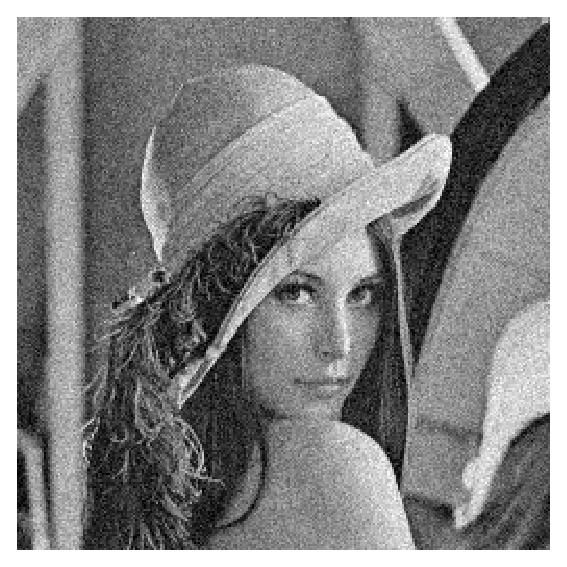
\includegraphics[width=0.48\linewidth]{denoising/lena-noisy.eps}&
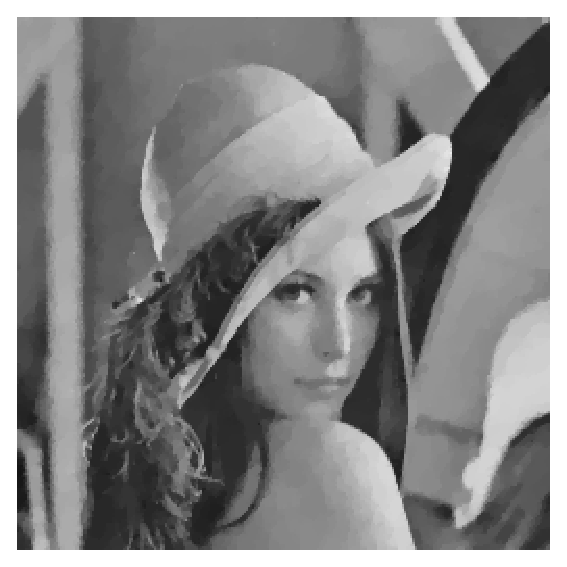
\includegraphics[width=0.48\linewidth]{denoising/lena-2.eps}\\
Noisy image $y$ & $f^\star$ with $\normTV{f_0}/\normTV{f^\star}=2$ \\[2mm]
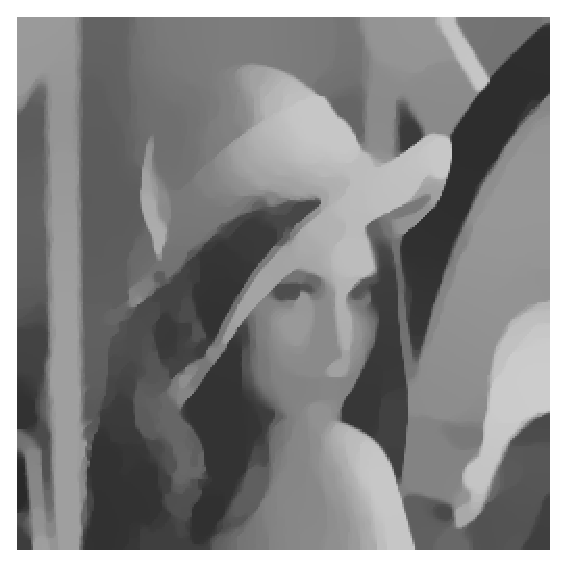
\includegraphics[width=0.48\linewidth]{denoising/lena-4.eps}&
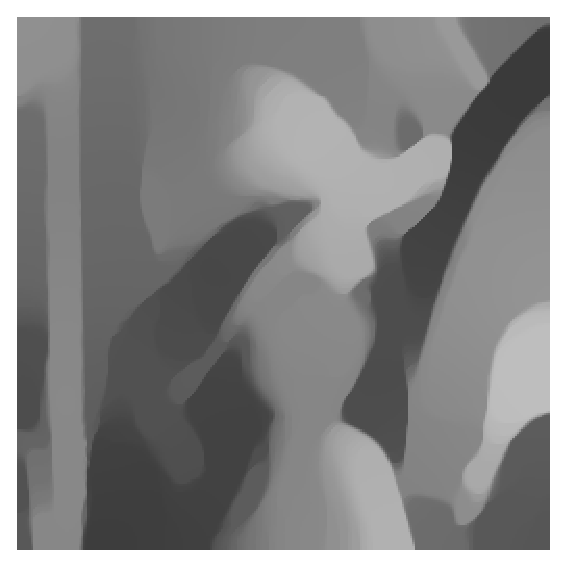
\includegraphics[width=0.48\linewidth]{denoising/lena-8.eps}\\
$f^\star$ with $\normTV{f_0}/\normTV{f^\star}=4$ & $f^\star$ with $\normTV{f_0}/\normTV{f^\star}=8$\\
\end{tabular}
}{ %
Examples of total variation projections computed with our algorithm. %
}{fig-denoising}


\myfigure{
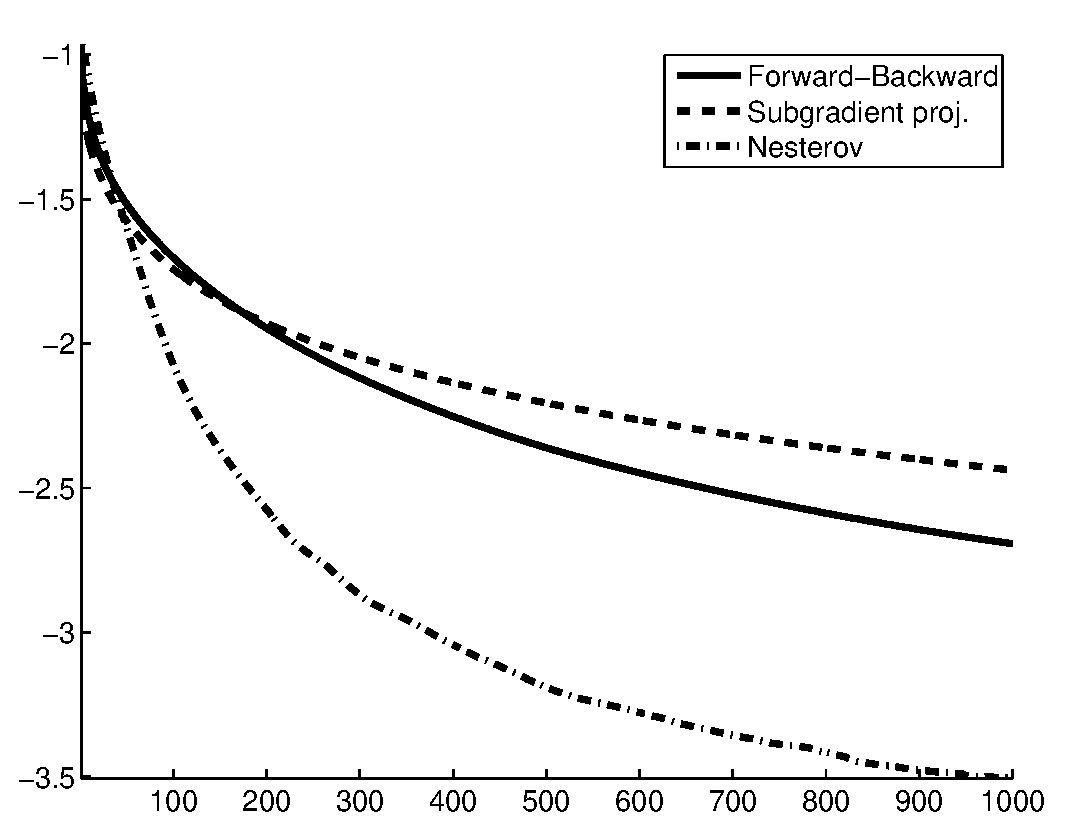
\includegraphics[width=0.8\linewidth]{errors/lena-l2-error.eps}
}{ %
Decay with $k$ of the error $\log_{10}( \norm{f^{(k)}-f^\star}/\norm{f^\star} )$ for the one-step forward-backward dual projection in Algorithm~\ref{algorithm-tv-proj} (solid line), for the multi-step dual projection in Algorithm~\ref{algorithm-tv-proj-nesterov} (dashed-dotted line),
and the sub-gradient projection \cite{combettes-pesquer-tv} (dashed line). Here $\tau = \normTV{f_0}/4$. %
}{fig-l2-error}


\myfigure{
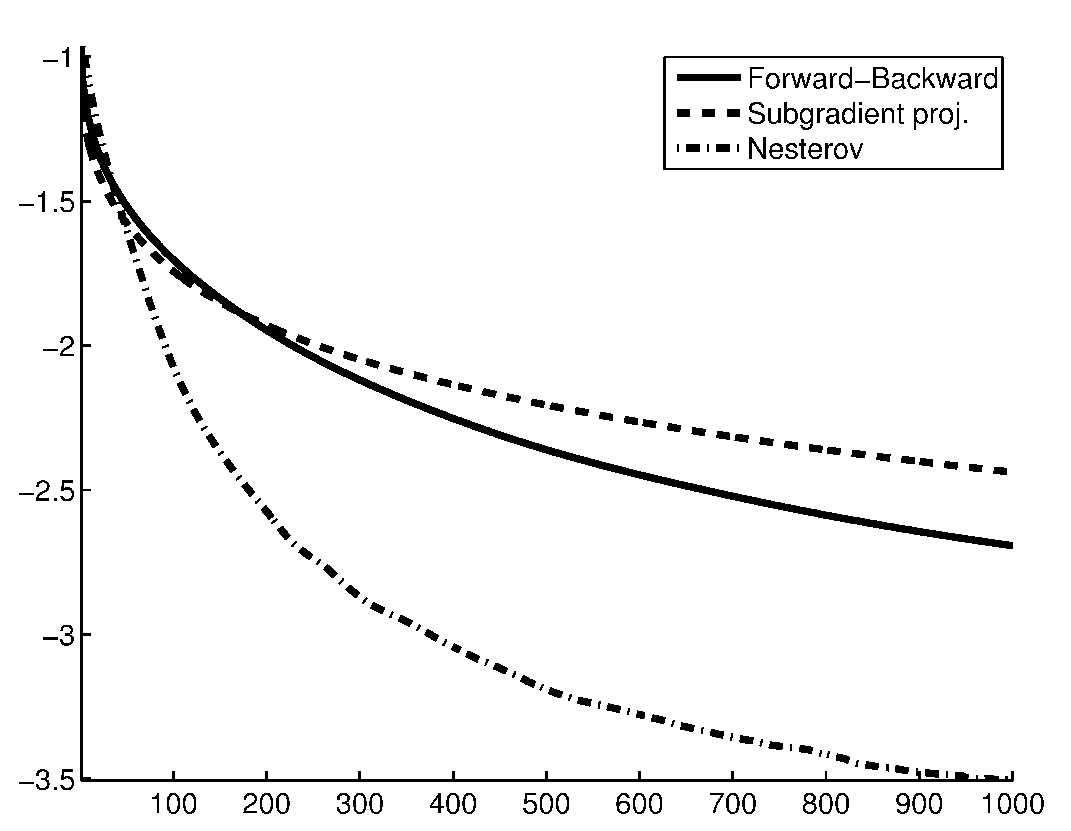
\includegraphics[width=0.8\linewidth]{errors/lena-tv-error.eps}
}{ %
Decay with $k$ of the total variation error $\log_{10}(\normTV{f^{(k)}}/\tau-1)$ for the same algorithms as in Figure~\ref{fig-l2-error}. Here $\tau = \normTV{f_0}/4$. %
}{fig-tv-error}



%%%%%%%%%%%%%%%%%%%%%%%%%%%%%%%%%%%%%%%%%%%%%%%%%%%%%%%%%%%%%%
\subsection{Total Variation Texture Synthesis}
\label{subsec-texture-synth}

Statistical approaches to texture synthesis draw an image at random from a set of potential textures defined by constraints that can be learned from an exemplar texture. A standard procedure considers the outputs of a filter-bank, such as wavelets, and constrains their marginal distributions to match those of the exemplar \cite{heeger-pyramid-texture,zhu-frame}. Instead of considering the uniform distribution inside the set of constraints--assumed to have a non-empty intersection-- and sample from this intersection, a simpler approach is to use alternating projections onto the constraints of an initial random white noise image \cite{portilla-parametric-model}. Although the constrained sets are often non-convex, hopefully, this scheme converges locally to a point within the intersection of the constraints that is expected to be visually similar to the exemplar image.

We propose here to consider a total variation constraint to better preserve sharp edges during the synthesis
\eq{
	\Cc_{\text{TV}} = \enscond{ f \in \RR^N }{ \normTV{f} \leq \tau } ~,
}
where $\tau$ might be computed from an exemplar texture $\tau = \normTV{f_0}$.
This constraint is especially suitable for piecewise-smooth textures representing objects occluding each other.

To enforce other statistical constraints as well, we set up a simple texture model where the mean and the standard deviation of the synthesized texture are preserved. Without loss of generality, the mean can be set to zero, and the standard deviation constraint amounts to the non-convex closed set
\eq{
	\Cc_{\text{std}} = \enscond{ f \in \RR^N }{  \norm{f - \bar{f}}/n = \beta }.
}
where $\bar{f} = \sum_{i,j=0}^{n-1} f[i,j]/N$ is the mean of $f$, and $\beta$ can be set from an exemplar $\beta = \norm{f_0 - \bar{f_0}}/n$. Clearly, in finite dimensions, the set $\Cc_{\text{std}}$ is a bounded sphere in $\RR^N$. The closed set $\Cc_{\text{std}}$ is prox-regular since its associated orthogonal projector is single-valued through the simple formula
\eql{\label{eq-histo-matching}
      \Proj_{\Cc_\text{std}}(f) = n\beta \left(f - \bar{f}\right)/\norm{f - \bar{f}} ~.
}
%the histogram of grayscale intensity is imposed. In a discrete setting, this amounts to selecting a set $V = \{ v_i \}_{ i=0 }^{N-1}$ of $N$ values $v_i \in \RR$, and consider the non-convex compact constraint set
%\eq{
%	\Cc_V = \enscond{ f \in \RR^N }{  \{ f[i,j] \}_{i,j=0}^{n-1} = V }.
%}
%In other words, the constraint $f \in \Cc_V$ imposes that the contrast of the texture remains the same during the synthesis. We note that more complicated statistical constraints can be imposed as well, see for instance \cite{portilla-parametric-model}.

The synthesis algorithm, detailed in Algorithm~\ref{algorithm-tv-synthesis}, corresponds to the von Neumann's method of alternating projections onto the two constraint sets 
\eq{
	f^{(\ell+1)} = \Proj_{\Cc_{\text{std}}}\pa{ \Proj_{\normTV{\cdot}\leq \tau}( f^{(\ell)} ) } ~,
}
starting from an initial noise texture $f^{(0)}$. 

{\linespread{1}
\begin{algorithm}[h]
\noindent{\bf{Initialization:}} set $f^{(0)} = $ random white noise and set $\ell=0$.\\
\noindent{\bf{Main iteration:}} \\
\While{$\norm{f^{(\ell+1)} - f^{(\ell)}} > \tol$}{
\begin{enumerate}
	\item \textit{Impose TV constraint:} compute 
		\eq{
			\tilde f^{(\ell)} = \Proj_{\normTV{\cdot}\leq \tau} f^{(\ell)}
		}
		using our dual projection Algorithm~\ref{algorithm-tv-proj} or \ref{algorithm-tv-proj-nesterov}.
	\item \textit{Impose histogram constraint:} compute 
		\eq{
			f^{(\ell+1)} = \Proj_{\Cc_{\text{std}}} \tilde f^{(\ell)}
		}
		where.
	\item $\ell \leftarrow \ell+1$.
\end{enumerate}}
    \caption{Total variation texture synthesis algorithm. \label{algorithm-tv-synthesis}}
\end{algorithm}}

% The orthogonal projection $\Proj_{\Cc_V}(f)$ of an image onto $\Cc_V$ corresponds to an histogram equalization. We assume that the values of $V$ are ordered by increasing values $v_i \leq v_{i+1}$, and we denote by $f[r(i)]$ the ordered values of $f$, where $r$ is a permutation of the pixel indices. The orthogonal projection is then
% \eql{\label{eq-histo-matching}
% 	\Proj_{\Cc_V}(f) = \tilde f
% 	\qwithq
% 	\tilde f[r(i)] = v_i.
% }

Using arguments from \cite{Lewis09}, we can conclude that our non-convex alternating projections algorithm for texture synthesis converges locally to a point of the intersection $\Cc_{\text{TV}} \cap \Cc_{\text{std}}$ which is non-empty as the exemplar $f_0$ is in it. Indeed, both constraint sets are closed and prox-regular, i.e. the associated orthogonal projectors are single-valued since $\Cc_{\text{TV}}$ is convex and $\Cc_{\text{std}}$ is a smooth manifold. Thus, by \cite[Corollary 5.18]{Lewis09}, Algorithm~\ref{algorithm-tv-synthesis} converges at a linear rate associated with a modulus of regularity depending on the geometry of the intersection, with the proviso that the latter is strongly regular; see \cite[Section 2]{Lewis09} for a definition of strong regularity. The legitimate question that one may ask is whether the above algorithm is robust with regard to the inexact computation of the projector onto $\Cc_{\text{TV}}$ which is obtained by running Algorithm~\ref{algorithm-tv-proj} or \ref{algorithm-tv-proj-nesterov} a finite number of iterations. It turns out that by virtue of \cite[Theorem 6.1]{Lewis09}, the convergence of Algorithm~\ref{algorithm-tv-synthesis} with the inexact projection on $\Cc_{\text{TV}}$ can still be guaranteed.

Figure~\ref{fig-synthesis} depicts examples of texture synthesis using Algorithm~\ref{algorithm-tv-synthesis}. The latter always converged in practice though we cannot guarantee in fact that the intersection of the two constraint sets is strongly regular. When the total variation constraint $\tau$ decreases, short edges are removed. This allows to interpolate between a noisy texture and a cartoon image with sharp edges. 
%where the pixel values $V$ are equally spaced in $[0,1]$ so that the textures have a uniform distribution of gray values. 

\myfigure{
\begin{tabular}{@{}c@{\hspace{2mm}}c@{}}
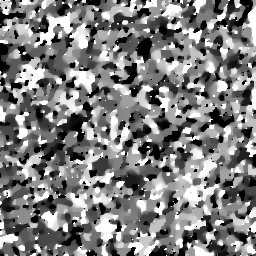
\includegraphics[width=0.48\linewidth]{synthesis/tv-synthesis-std-4}&
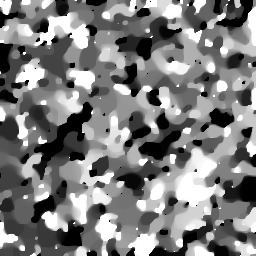
\includegraphics[width=0.48\linewidth]{synthesis/tv-synthesis-std-8}\\
$\normTV{f^{(0)}}/\normTV{f^\star}=4$ & $\normTV{f^{(0)}}/\normTV{f^\star}=8$ \\[2mm]
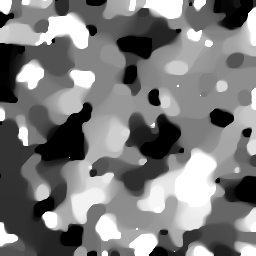
\includegraphics[width=0.48\linewidth]{synthesis/tv-synthesis-std-16}&

\includegraphics[width=0.48\linewidth]{synthesis/tv-synthesis-std-32}\\
$\normTV{f^{(0)}}/\normTV{f^\star}=16$ & $\normTV{f^{(0)}}/\normTV{f^\star}=32$
\end{tabular}
}{ %
Texture synthesis with TV projection and standard deviation constraint. %
}{fig-synthesis}

%%%%%%%%%%%%%%%%%%%%%%%%%%%%%%%%%%%%%%%%%%%%%%%%%%%%%%%%%%%%%%
\subsection{Inpainting}
\label{subsec-inpainting}

Inpainting aims at restoring an image $f_0$ from which a set $\Om \subset \{0,\ldots,n-1\}^2$ of pixels is missing. It corresponds to the inversion of the ill-posed linear problem \eqref{eq-ip-inversion} where $\Phi$ is defined as
\eql{\label{eq-inpainting-pbm}
		(\Phi f)[i,j] = 
		\begin{cases}
			0      &\qifq (i,j) \in \Omega,\\
			f[i,j] &\qifq (i,j) \notin \Omega.
		\end{cases}
}
In this case, it is obvious that $\opnorm{\Phi}=1$, and we use $\nu=1$ for the projected gradient descent Algorithm~\ref{algorithm-tv-ip}. The recursion \eqref{eq-proj-grad} amounts to first imposing the known values outside $\Om$
\eq{
	\tilde f^{(\ell)}[i,j] = 
	\choice{
		f^{(\ell)}[i,j] \qifq (i,j) \in \Om,\\
		y[i,j] \text{ otherwise}. 
	}
}
and then projecting onto the TV ball
\eq{
	f^{(\ell+1)} = \Proj_{\{\normTV{\cdot} \leq \tau\}} \tilde f^{(\ell)}.
}

The top of Figure~\ref{fig-ip-tv}, exemplifies a damaged image $y$ of $N = 512^2$ pixels, with $|\Om|/N=0.7$ of randomly removed pixels. The noise is AWGN with standard deviation $0.05\normi{f_0}$. 

The inpainted image $f^\star$ (output PSNR=25.67 dB) is computed by solving \eqref{tvproj-ip-constr} with the projected gradient descent, Algorithm~\ref{algorithm-tv-ip}, with a total variation constraint size $\tau = 0.6 \normTV{f_0}$. The number of iterations for the projection step 3) is controlled by setting $\tol_{\text{proj}}=10^{-2}$. Roughly between 10 to 20 iterations of dual projections are required to maintain the total variation constraints during the gradient descent. Figure~\ref{fig-ip-convergence}, top, depicts the decay in log scale of the iterates error, that exhibits a roughly linear convergence speed for large $\ell$. This rate is likely to be a consequence of the special structure of the masking operator $\Phi$. We think that this can justified in the light of compressed sensing arguments (the mask is random here), and the convergence analysis in \cite{BrediesLorentz08}. We leave these aspects, which are beyond the scope of the paper, to a future work.


%%%%%%%%%%%%%%%%%%%%%%%%%%%%%%%%%%%%%%%%%%%%%%%%%%%%%%%%%%%%%%
\subsection{Deconvolution}
\label{subsec-deconvolution}

An optical system produces a blur that is modeled by convolution with a low pass point spread function (PSF) $\phi$. In such a case, the operator $\Phi$ in \eqref{eq-ip-inversion} represents the circular convolution with $\varphi$. The convolution by $\phi$ removes high frequency details and the total variation constraint \eqref{tvproj-ip-constr} helps to recover sharp edges of the original image. 

Figure~\ref{fig-ip-convergence}, bottom, gives an example of blurred image $y$ of $N = 512^2$ pixels. The PSF is a Gaussian kernel 
of standard deviation $s=4$ pixels, normalized to a unit mass. Thus $\opnorm{\Phi}=1$. The noise is AWGN with standard deviation $0.02\norm{f_0}_{\infty}$. We use a gradient descent step-size $\nu=1.9$ in Algorithm~\ref{algorithm-tv-ip}.

The deconvolved image $f^\star$ (output PSNR=24.48 dB) is computed by applying Algorithm~\ref{algorithm-tv-ip} to $y$, with a total variation constraint size $\tau = 0.6 \normTV{f_0}$. Figure~\ref{fig-ip-convergence}, bottom, shows the decay in log scale of the iterates error. This is consistent with the predicted convergence rate of Theorem~\ref{theo:projdescent}.

\myfigurestar{
\begin{tabular}{@{}c@{\hspace{2mm}}c@{\hspace{2mm}}c@{}}
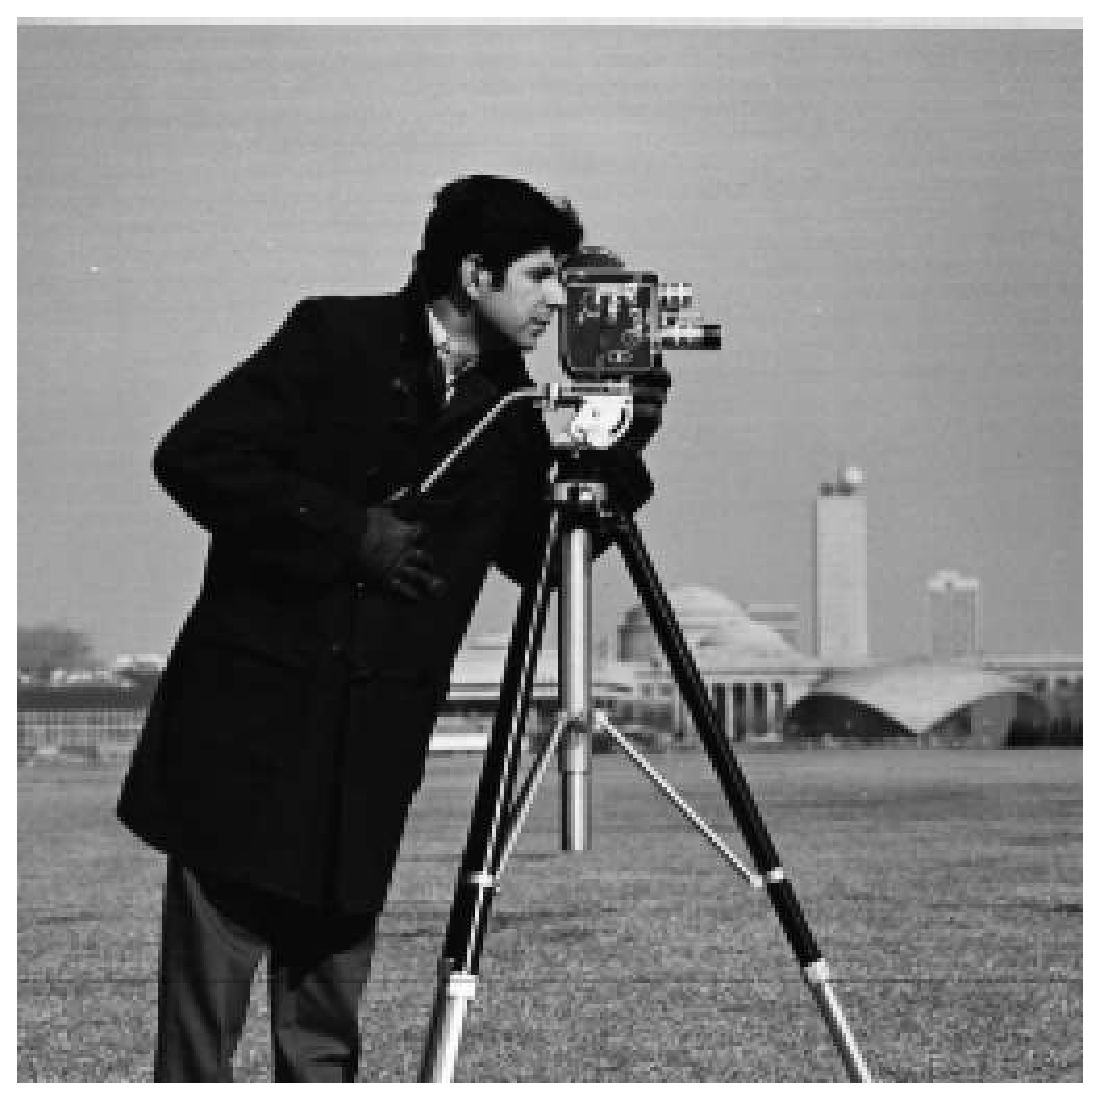
\includegraphics[width=0.32\linewidth]{inpainting/cameraman-inpainting-original.eps}&
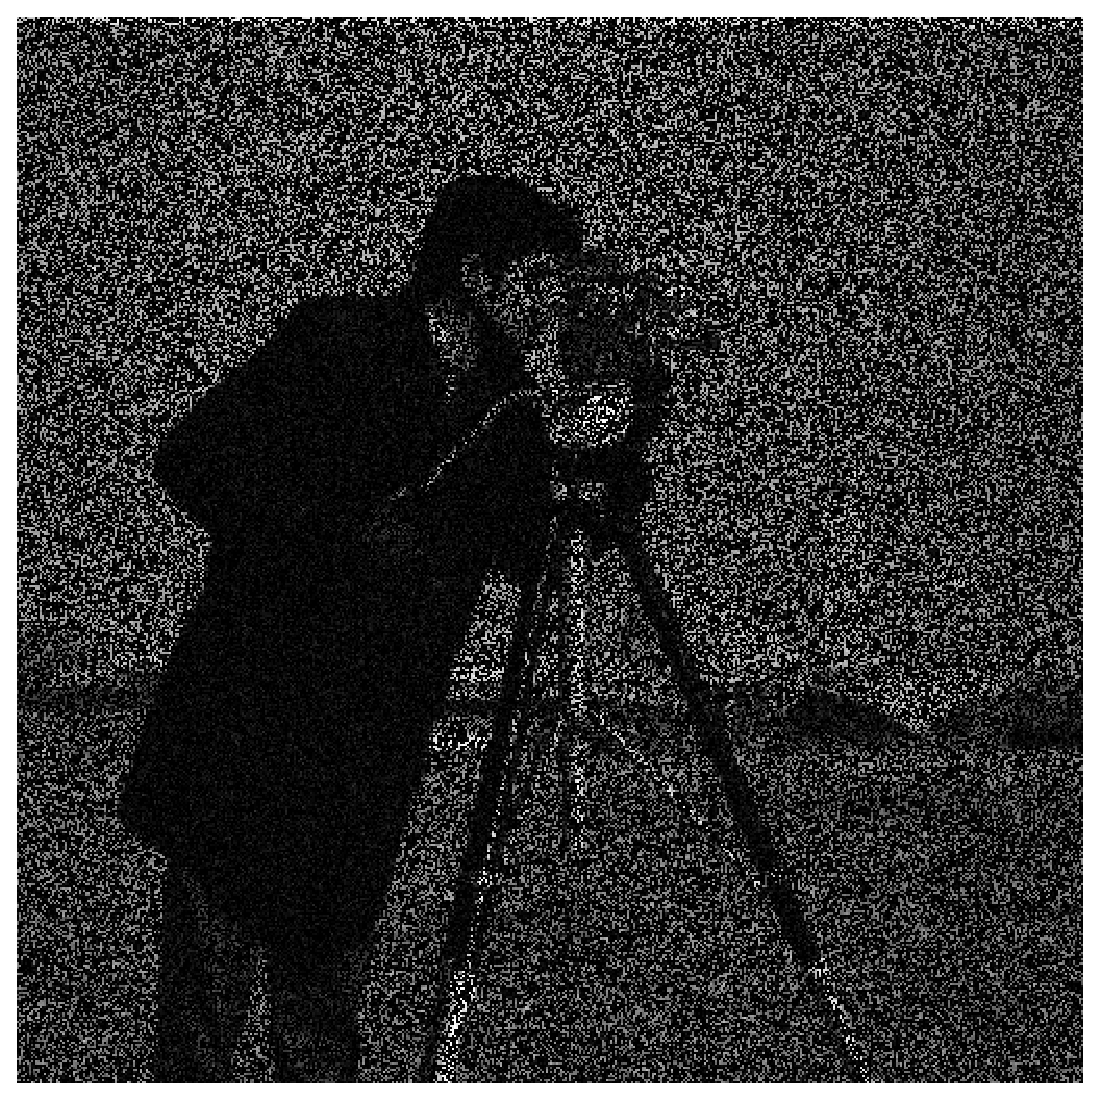
\includegraphics[width=0.32\linewidth]{inpainting/cameraman-inpainting-observation.eps}&
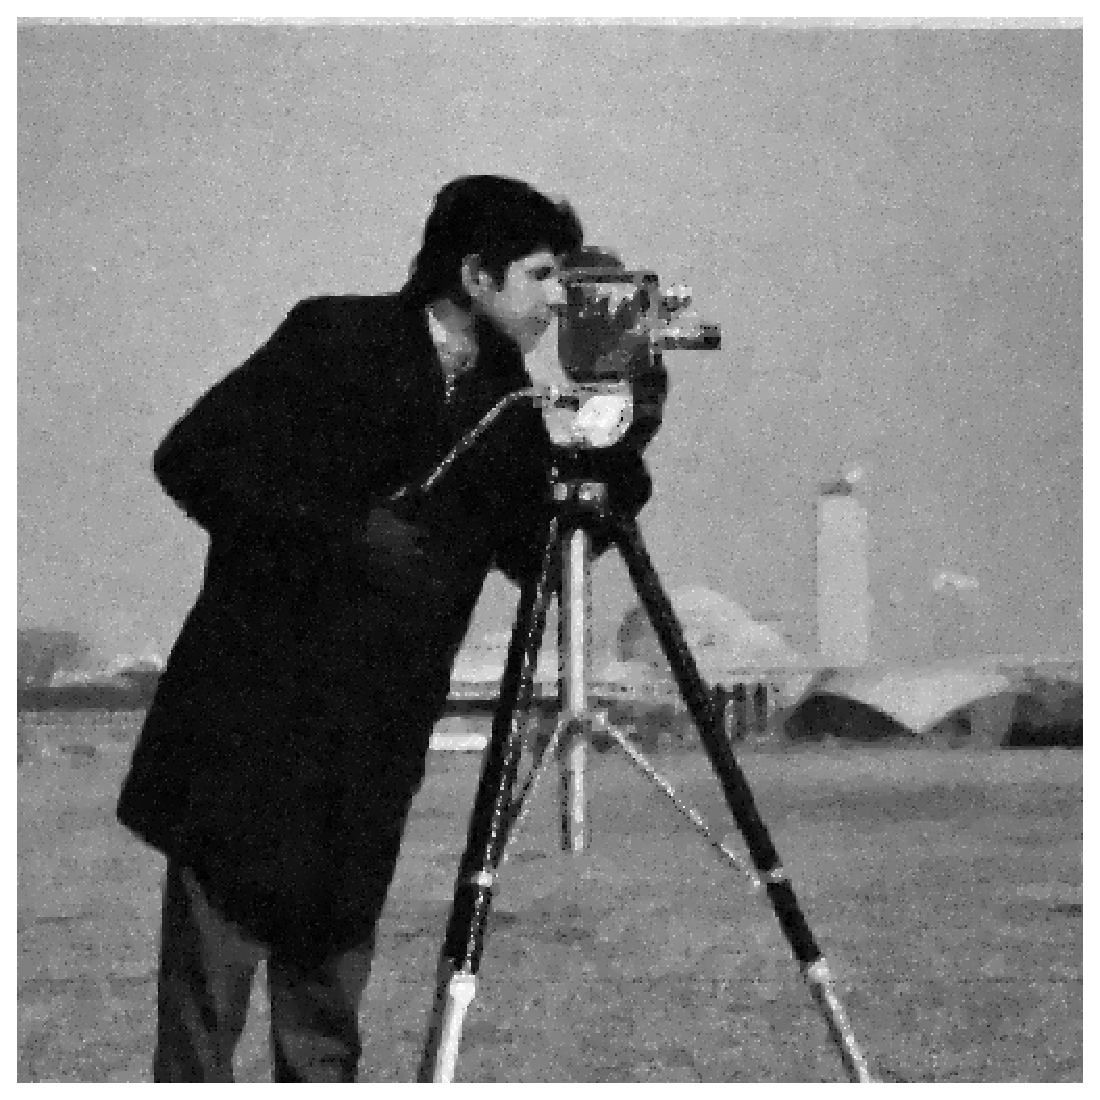
\includegraphics[width=0.32\linewidth]{inpainting/cameraman-inpainting-solution.eps}\\[1mm]
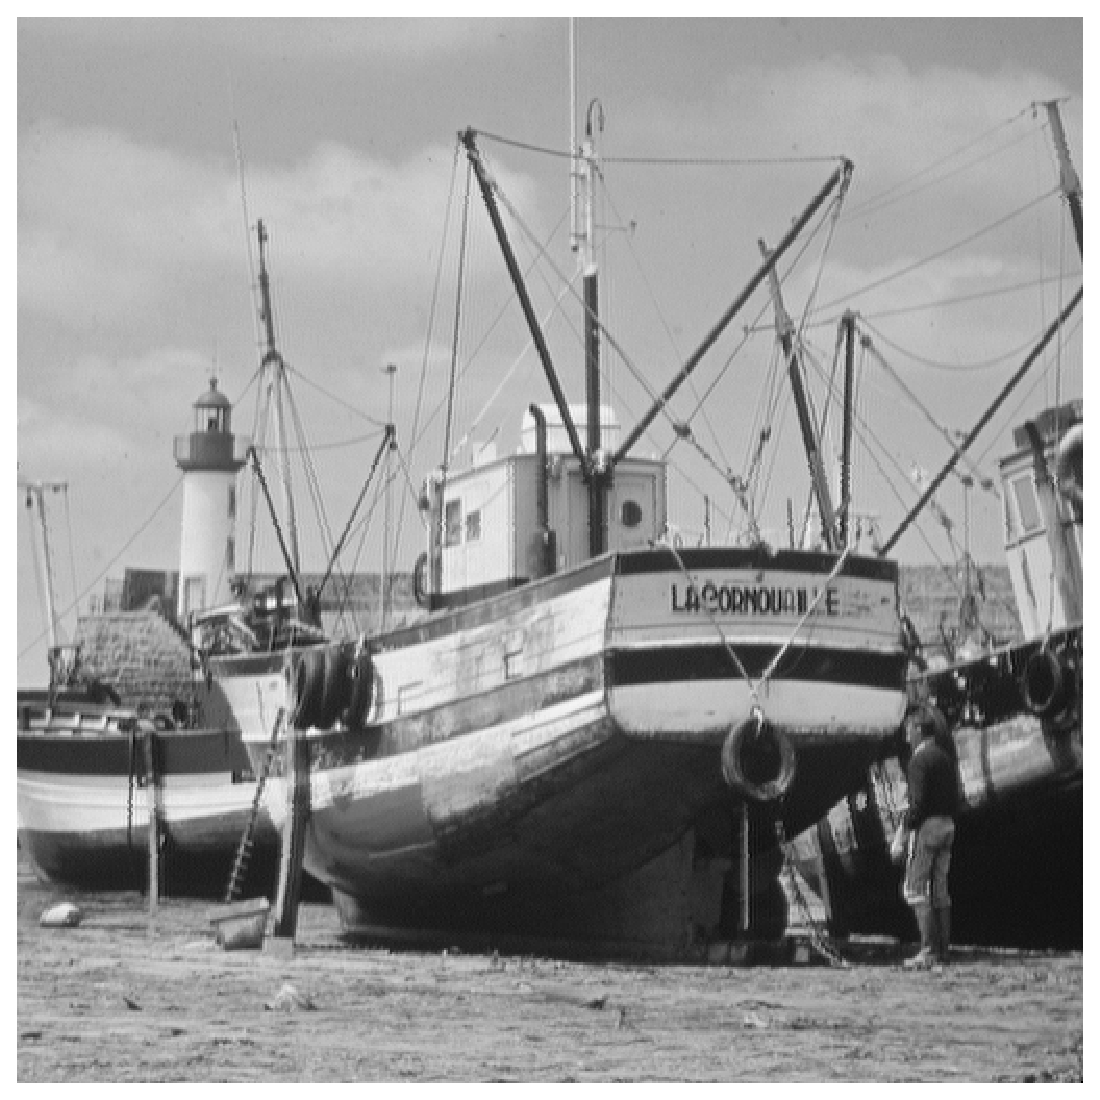
\includegraphics[width=0.32\linewidth]{deblurring/boat-deblurring-original.eps}&
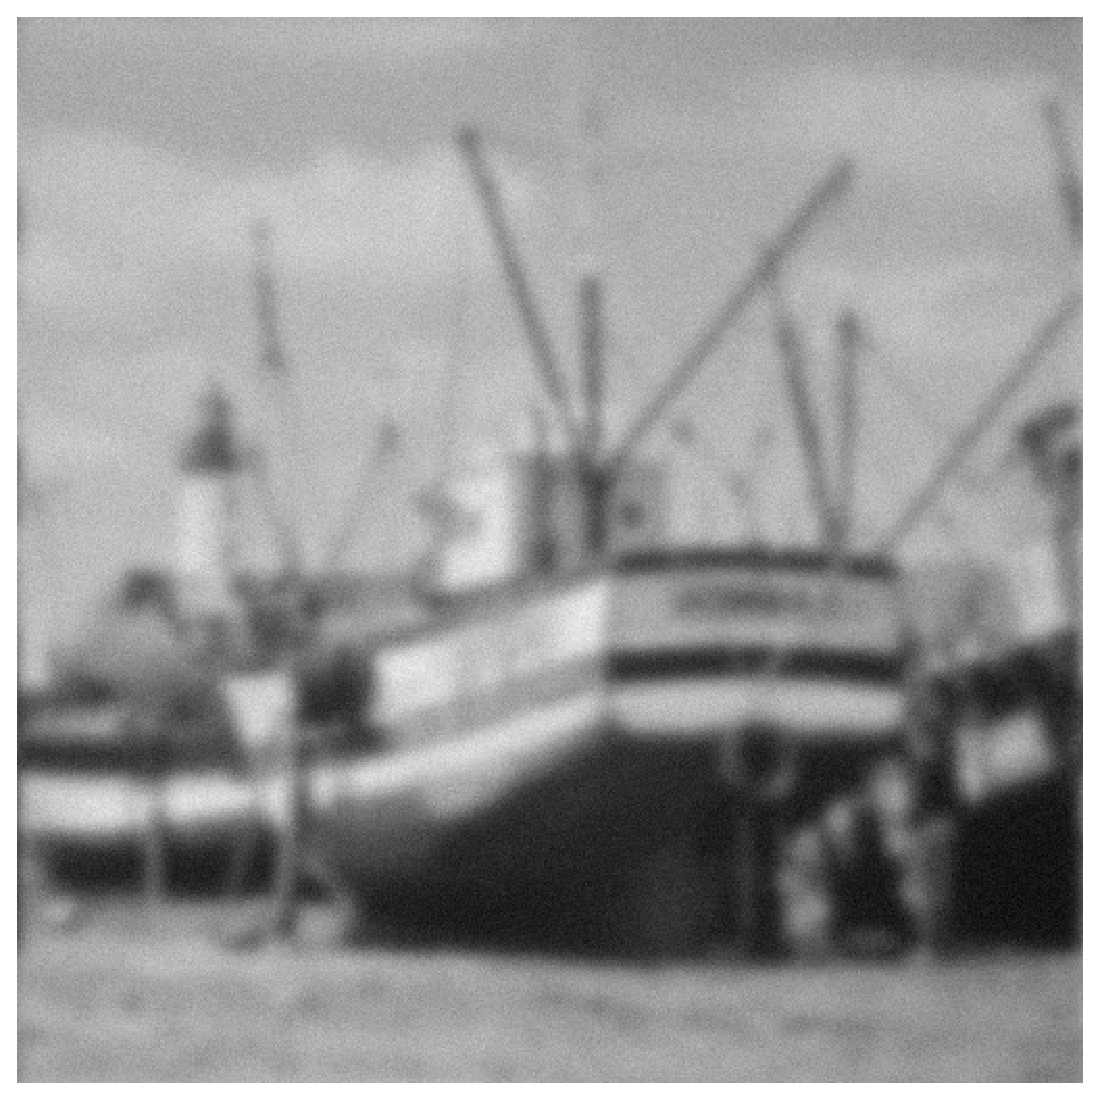
\includegraphics[width=0.32\linewidth]{deblurring/boat-deblurring-observation.eps}&
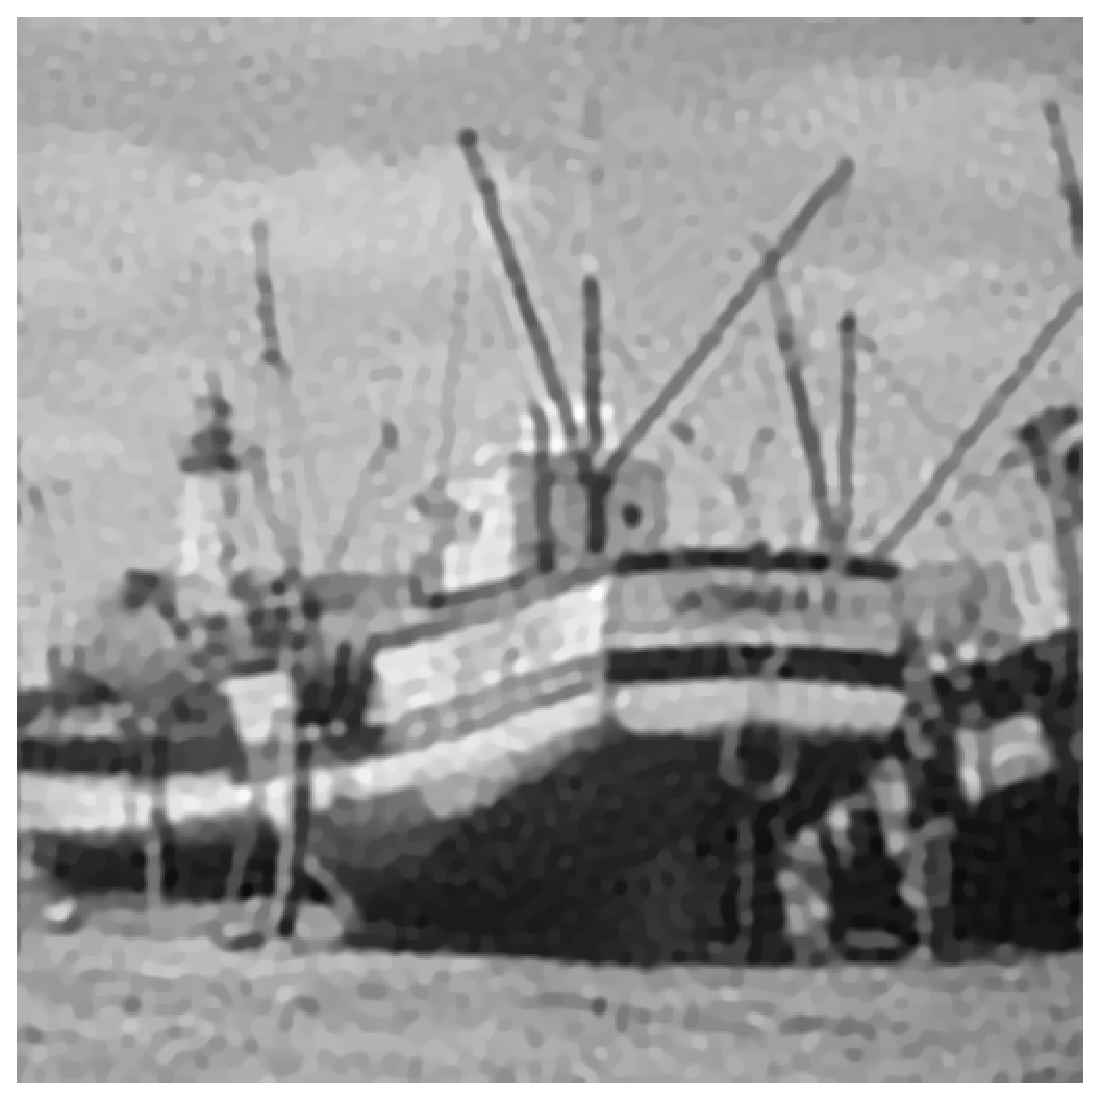
\includegraphics[width=0.32\linewidth]{deblurring/boat-deblurring-solution.eps}\\%[1mm]
$f_0$ & $y=\Phi f_0+\epsilon$ & $f^\star$ 
\end{tabular}
}{ %
Examples of inpainting (first row) and deconvolution (bottom row) using the TV constraint. %
}{fig-ip-tv}


\myfigure{
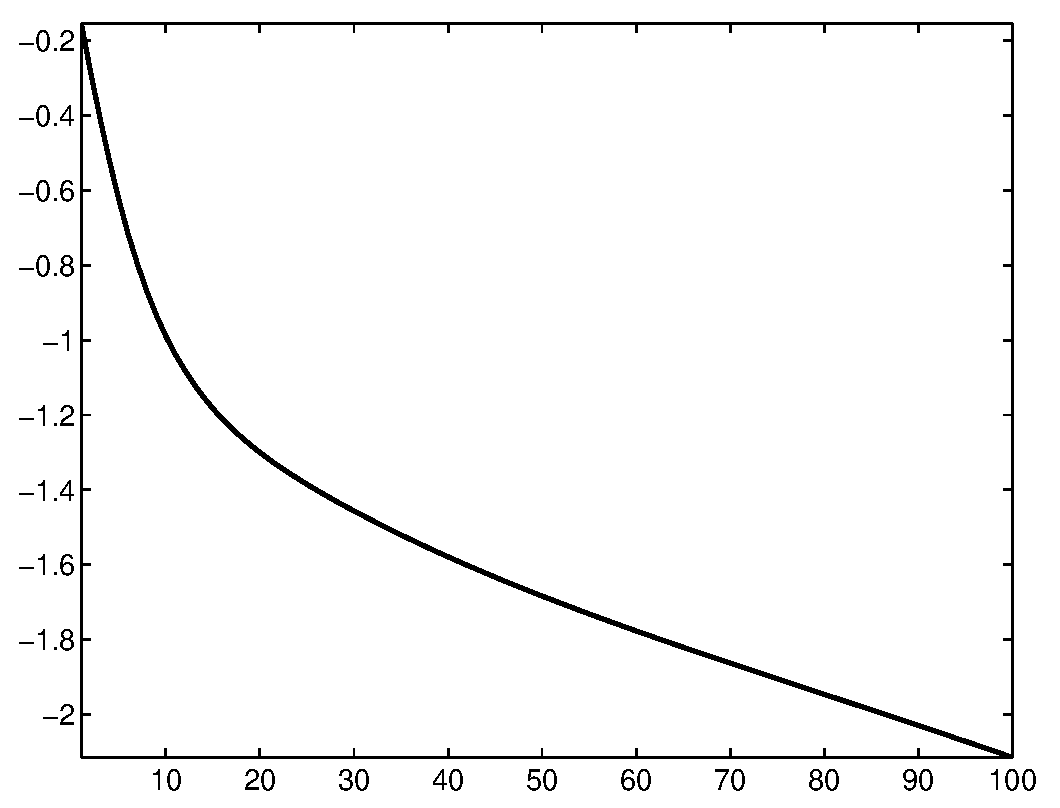
\includegraphics[width=0.8\linewidth]{inpainting/cameraman-inpainting-error.eps}\\\vspace{2mm}
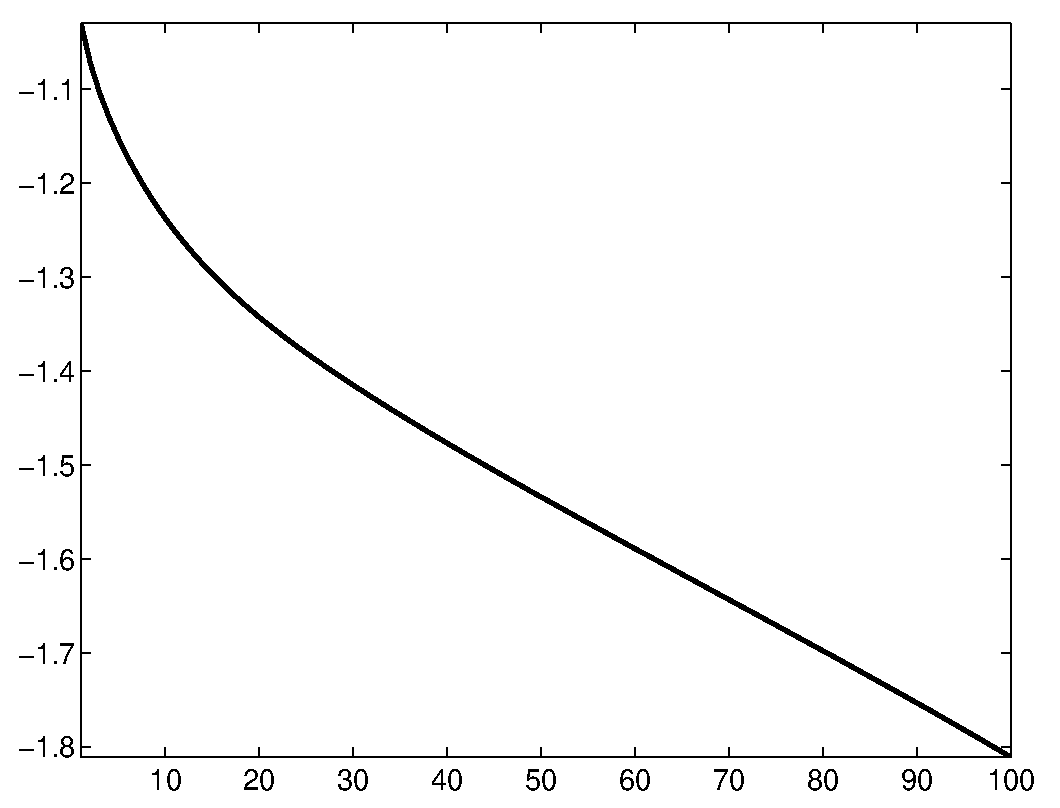
\includegraphics[width=0.8\linewidth]{deblurring/boat-deblurring-error.eps}
}{ %
Decay of the error $\log_{10}( \norm{f^{(\ell)}-f^\star} / \norm{f_0} )$ for inpainting (top) and
deconvolution (bottom). %
}{fig-ip-convergence}


%%%%%%%%%%%%%%%%%%%%%%%%%%%%%%%%%%%%%%%%%%%%%%%%%%%%%%%%%%%%%%
%%%%%%%%%%%%%%%%%%%%%%%%%%%%%%%%%%%%%%%%%%%%%%%%%%%%%%%%%%%%%%
%%%%%%%%%%%%%%%%%%%%%%%%%%%%%%%%%%%%%%%%%%%%%%%%%%%%%%%%%%%%%%
\section{Conclusion}

This paper proposes a new approach to compute the projection of an image on a total variation ball. This approach solves an unconstrained dual formulation of the primal problem, and boils down to an iterative soft thresholding on the gradient field. Two algorithms for solving the dual minimization problem were proposed. We also studied their convergence behavior and established their convergence rates.

Even though we only focused on the total variation norm in the constraint, our dualization-based projection approach is quite general and extends to any positively 1-homogeneous functional for which the conjugate can be easily computed. This includes constraints involving functionals of the form $\normu{G f}$ for any linear operator $G$ (of explicit adjoint) such as the analysis operator of a frame. The scheme also generalizes very easily to arbitrary dimension.
In particular, our proof of convergence rate on the forward-backward can be extended to the infinite dimensional case. It is also worth mentioning that the alternating-direction method of multipliers (ADMM) \cite{Glowinski89} can be used to solve \eqref{tv-proj-cont} by minimizing the augmented Lagrangian form, associated to a doubly constrained reformulation of \eqref{tv-proj-cont} through an auxiliary variable $w=\nabla f$, alternately over $w$ and $f$. Though no convergence rate is known for such an algorithm in general.

We have illustrated the projection algorithm over several applications such as denoising when little is known about the noise statistics, or to enforce total variation constraint in texture synthesis.  

A projected gradient descent was also proposed that uses this projection to solve linear inverse problems under a total variation constraint. Our projector can be advantageously used when additional constraints are involved, such as for example contrast bounds $a \leq f \leq b$ or affine constraints $A f = g$. Such a problem with compound constraints can be solved for instance using e.g. Douglas-Rachford splitting and its extensions.


\paragraph*{Acknowledgment}
The authors would like to thank Pierre Weiss for reading an earlier version of this paper and for fruitful discussions. This work is supported by ANR grant ANR-08-EMER-009.

%%%%%%%%%%%%%%%%%%%%%%%%%%%%%%%%%%%%%%%%%%%%%%%%%%%%%%%%%%%%%%
%%%%%%%%%%%%%%%%%%%%%%%%%%%%%%%%%%%%%%%%%%%%%%%%%%%%%%%%%%%%%%
%%%%%%%%%%%%%%%%%%%%%%%%%%%%%%%%%%%%%%%%%%%%%%%%%%%%%%%%%%%%%%
\bibliographystyle{IEEEtran} 
\bibliography{bibliography}


 
 
\end{document}
